\hypertarget{relationships}{%
\chapter{Relationships}\label{relationships}}

This chapter explores relationships between variables.

\begin{itemize}
\item
  We will visualize relationships using scatter plots, box plots, and
  violin plots,
\item
  And we will quantify relationships using correlation and simple
  regression.
\end{itemize}

The most important lesson in this chapter is that you should always
visualize the relationship between variables before you try to quantify
it; otherwise, you are likely to be misled.

\hypertarget{exploring-relationships}{%
\section{Exploring relationships}\label{exploring-relationships}}

So far we have only looked at one variable at a time. Now it's time to
explore relationships between variables. As a first example, we'll look
at the relationship between height and weight.

We'll use data from the Behavioral Risk Factor Surveillance System
(BRFSS), which is run by the Centers for Disease Control at
\url{https://www.cdc.gov/brfss}. The survey includes more than 400,000
respondents, but to keep things manageable, I've selected a random
subsample of 100,000.

\begin{lstlisting}[language=Python,style=source]
import pandas as pd

brfss = pd.read_hdf('brfss.hdf5', 'brfss')
brfss.shape
\end{lstlisting}

\begin{lstlisting}[style=output]
(100000, 9)
\end{lstlisting}

Here are the first few rows.

\begin{lstlisting}[language=Python,style=source]
brfss.head()
\end{lstlisting}

\begin{tabular}{lrrrrrrrrr}
\toprule
{} &  SEX &   HTM4 &   WTKG3 &  INCOME2 &       \_LLCPWT &  \_AGEG5YR &  \_VEGESU1 &  \_HTMG10 &   AGE \\
\midrule
96230  &  2.0 &  160.0 &   60.33 &      8.0 &   1398.525290 &       6.0 &      2.14 &    150.0 &  47.0 \\
244920 &  2.0 &  163.0 &   58.97 &      5.0 &     84.057503 &      13.0 &      3.14 &    160.0 &  89.5 \\
57312  &  2.0 &  163.0 &   72.57 &      8.0 &    390.248599 &       5.0 &      2.64 &    160.0 &  42.0 \\
32573  &  2.0 &  165.0 &   74.84 &      1.0 &  11566.705300 &       3.0 &      1.46 &    160.0 &  32.0 \\
355929 &  2.0 &  170.0 &  108.86 &      3.0 &    844.485450 &       3.0 &      1.81 &    160.0 &  32.0 \\
\bottomrule
\end{tabular}

The BRFSS includes hundreds of variables. For the examples in this
chapter, I chose just nine. The ones we'll start with are
\passthrough{\lstinline!HTM4!}, which records each respondent's height
in cm, and \passthrough{\lstinline!WTKG3!}, which records weight in kg.

\begin{lstlisting}[language=Python,style=source]
height = brfss['HTM4']
weight = brfss['WTKG3']
\end{lstlisting}

To visualize the relationship between these variables, we'll make a
\textbf{scatter plot}. Scatter plots are common and readily understood,
but they are surprisingly hard to get right.

As a first attempt, we'll use \passthrough{\lstinline!plot!} with the
style string \passthrough{\lstinline!o!}, which plots a circle for each
data point.

\begin{lstlisting}[language=Python,style=source]
import matplotlib.pyplot as plt

plt.plot(height, weight, 'o')

plt.xlabel('Height in cm')
plt.ylabel('Weight in kg')
plt.title('Scatter plot of weight versus height');
\end{lstlisting}

\begin{center}
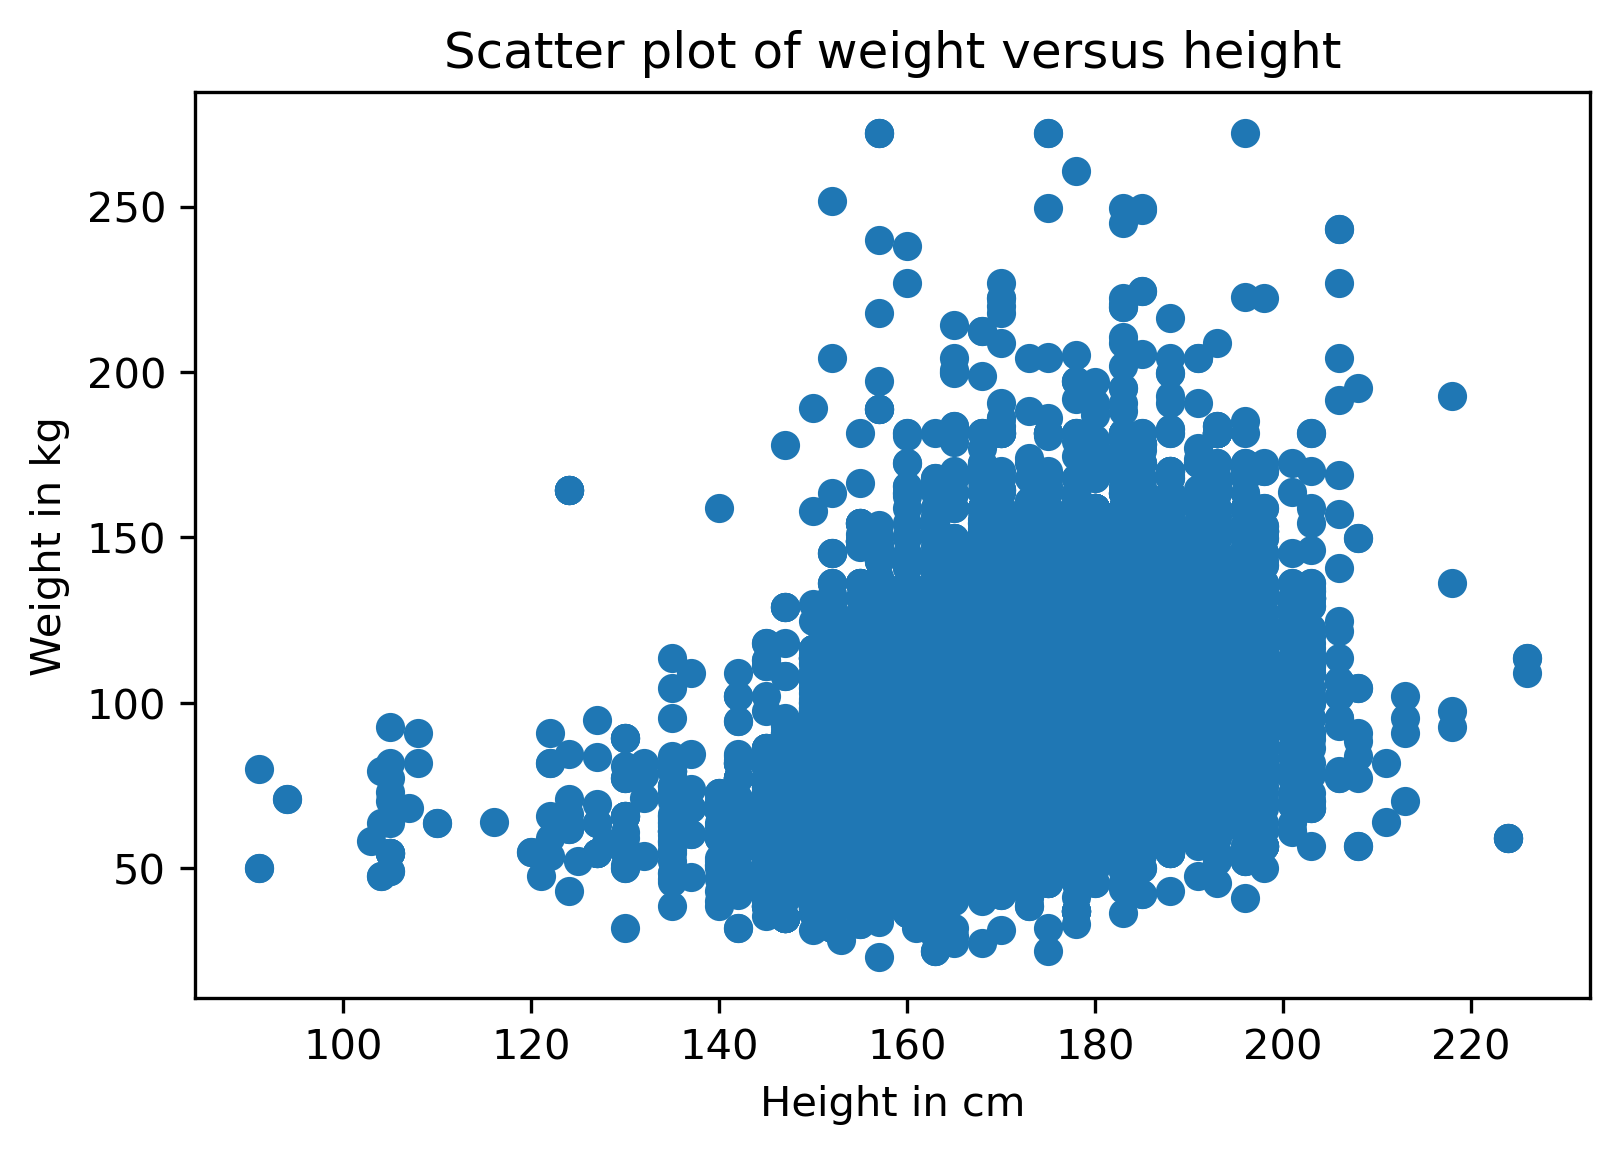
\includegraphics[scale=0.75]{09_relationships_files/09_relationships_13_0.png}
\end{center}

In general, it looks like taller people are heavier, but there are a few
things about this scatter plot that make it hard to interpret. Most
importantly, it is \textbf{overplotted}, which means that there are data
points piled on top of each other so you can't tell where there are a
lot of points and where there is just one. When that happens, the
results can be seriously misleading.

One way to improve the plot is to use transparency, which we can do with
the keyword argument \passthrough{\lstinline!alpha!}. The lower the
value of alpha, the more transparent each data point is.

Here's what it looks like with \passthrough{\lstinline!alpha=0.02!}.

\begin{lstlisting}[language=Python,style=source]
plt.plot(height, weight, 'o', alpha=0.02)

plt.xlabel('Height in cm')
plt.ylabel('Weight in kg')
plt.title('Scatter plot of weight versus height');
\end{lstlisting}

\begin{center}
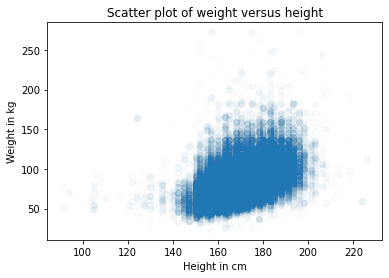
\includegraphics[scale=0.75]{09_relationships_files/09_relationships_15_0.png}
\end{center}

This is better, but there are so many data points, the scatter plot is
still overplotted. The next step is to make the markers smaller. With
\passthrough{\lstinline!markersize=1!} and a low value of alpha, the
scatter plot is less saturated. Here's what it looks like.

\begin{lstlisting}[language=Python,style=source]
plt.plot(height, weight, 'o', alpha=0.02, markersize=1)

plt.xlabel('Height in cm')
plt.ylabel('Weight in kg')
plt.title('Scatter plot of weight versus height');
\end{lstlisting}

\begin{center}
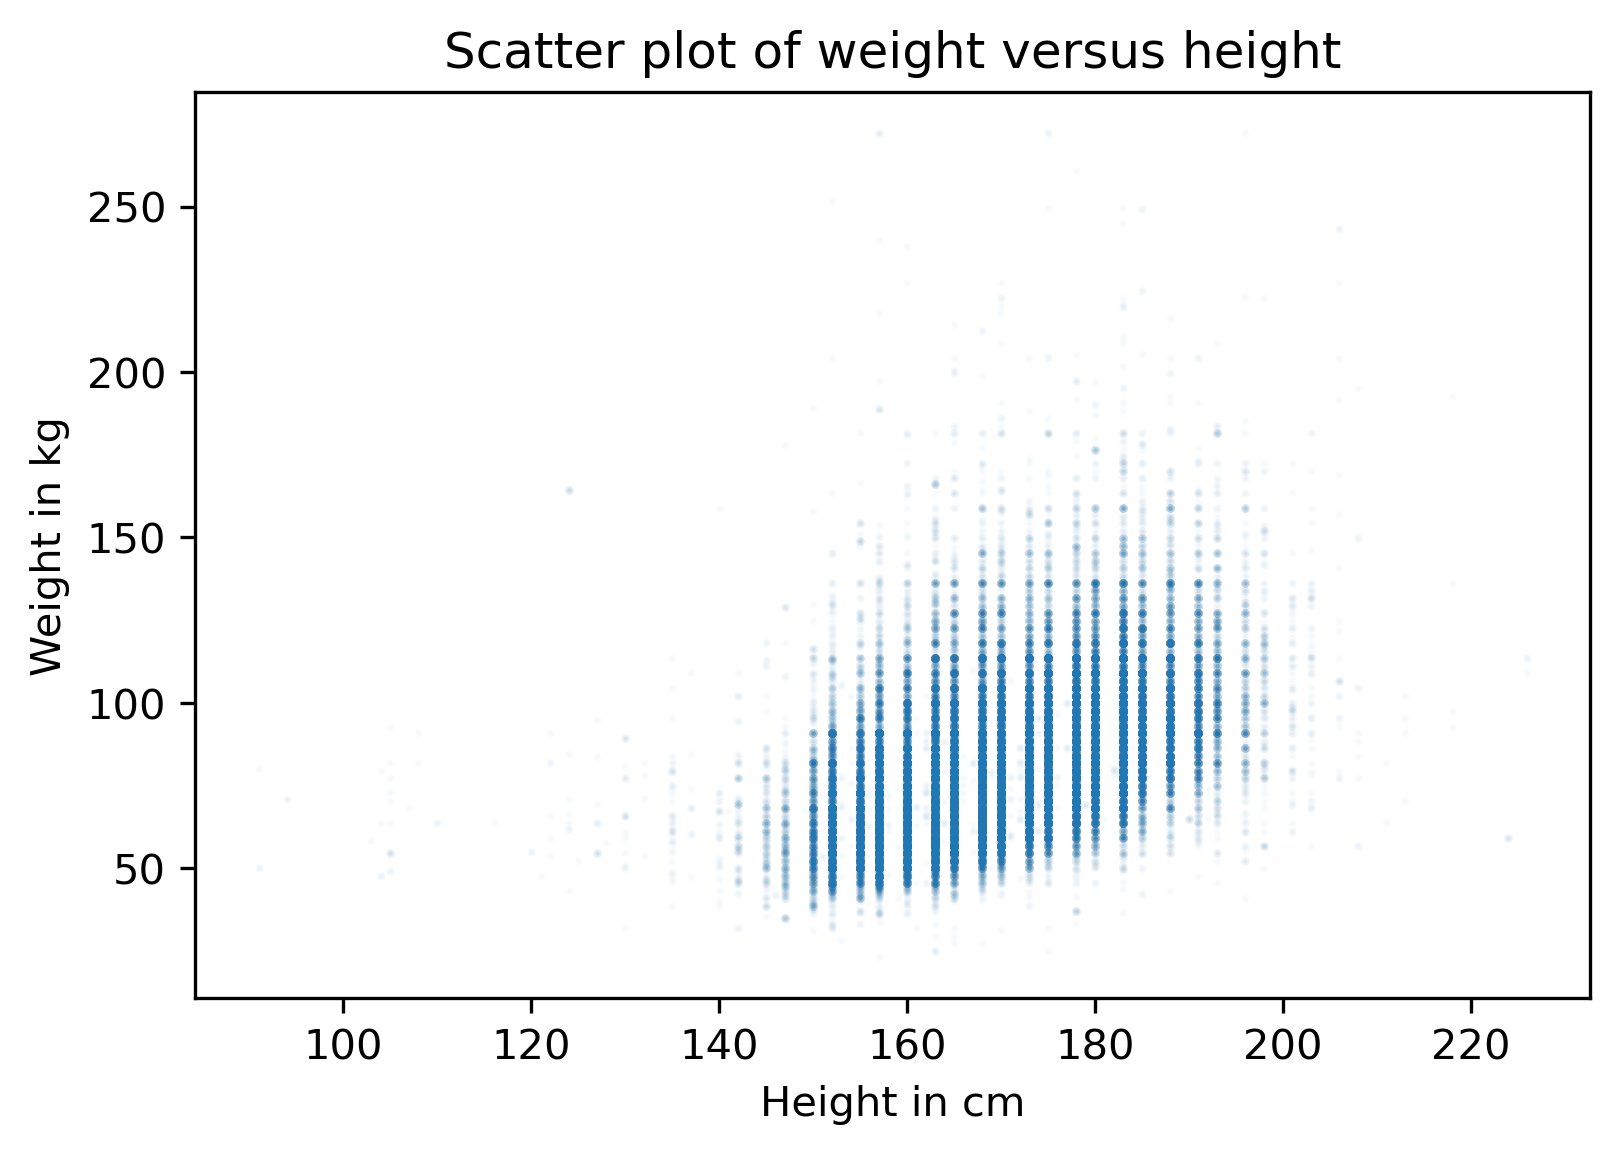
\includegraphics[scale=0.75]{09_relationships_files/09_relationships_17_0.png}
\end{center}

Again, this is better, but now we can see that the points fall in
discrete columns. That's because most heights were reported in inches
and converted to centimeters. We can break up the columns by adding some
random noise to the values; in effect, we are filling in the values that
got rounded off. Adding random noise like this is called
\textbf{jittering}.

We can use NumPy to add noise from a normal distribution with mean 0 and
standard deviation 2.

\begin{lstlisting}[language=Python,style=source]
import numpy as np

noise = np.random.normal(0, 2, size=len(brfss))
height_jitter = height + noise
\end{lstlisting}

Here's what the plot looks like with jittered heights.

\begin{lstlisting}[language=Python,style=source]
plt.plot(height_jitter, weight, 'o', 
         alpha=0.02, markersize=1)

plt.xlabel('Height in cm')
plt.ylabel('Weight in kg')
plt.title('Scatter plot of weight versus height');
\end{lstlisting}

\begin{center}
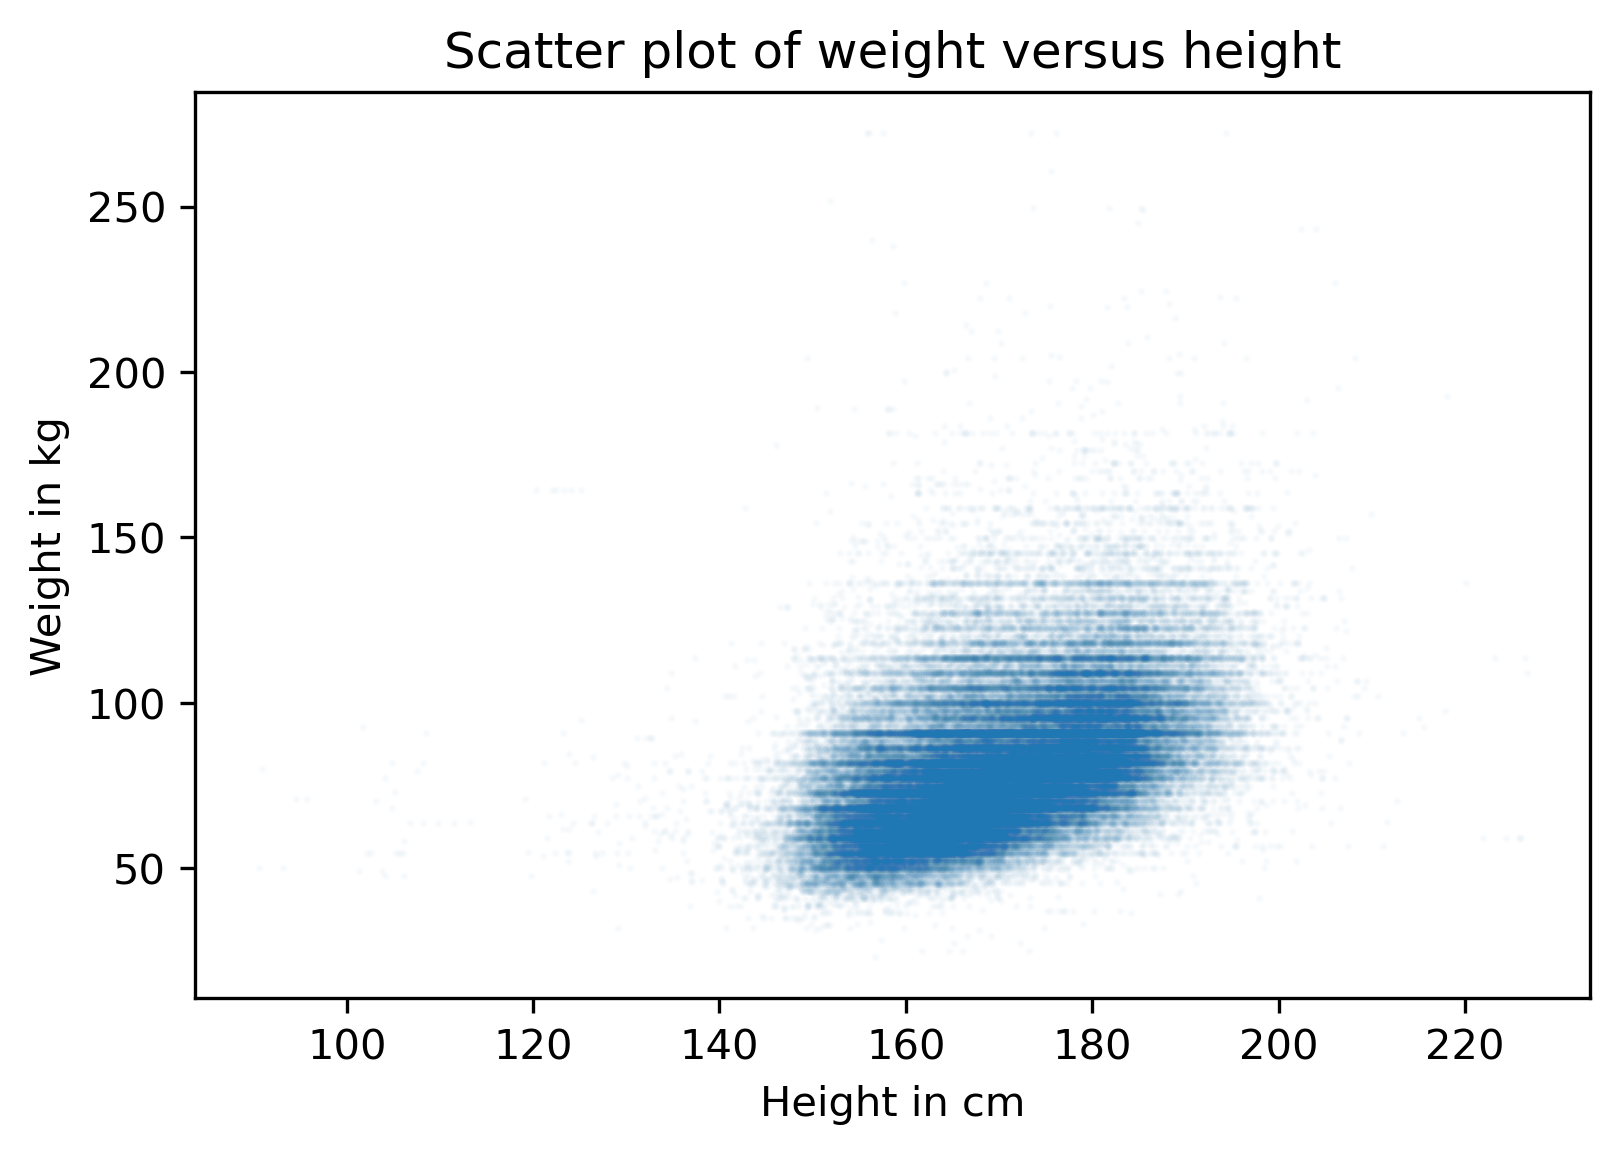
\includegraphics[scale=0.75]{09_relationships_files/09_relationships_21_0.png}
\end{center}

The columns are gone, but now we can see that there are rows where
people rounded off their weight. We can fix that by jittering weight,
too.

\begin{lstlisting}[language=Python,style=source]
noise = np.random.normal(0, 2, size=len(brfss))
weight_jitter = weight + noise
\end{lstlisting}

\begin{lstlisting}[language=Python,style=source]
plt.plot(height_jitter, weight_jitter, 'o', 
         alpha=0.02, markersize=1)

plt.xlabel('Height in cm')
plt.ylabel('Weight in kg')
plt.title('Scatter plot of weight versus height');
\end{lstlisting}

\begin{center}
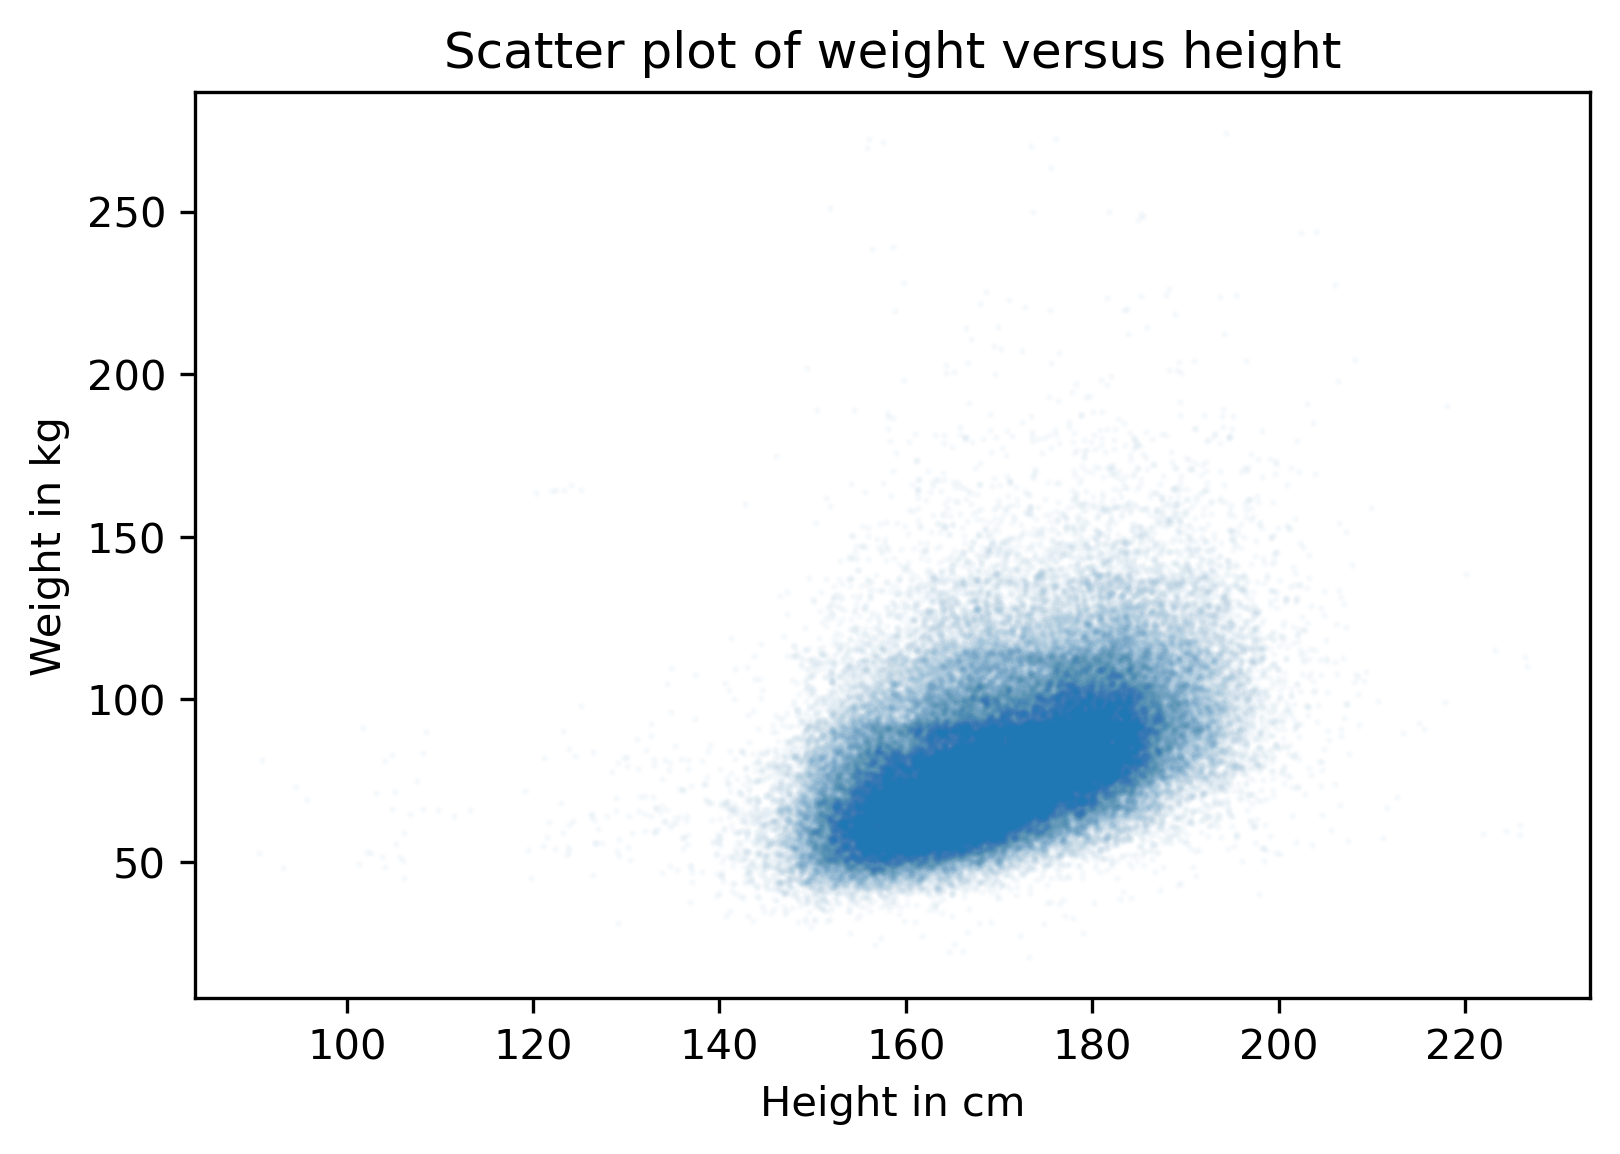
\includegraphics[scale=0.75]{09_relationships_files/09_relationships_24_0.png}
\end{center}

Finally, let's zoom in on the area where most of the data points are.

The functions \passthrough{\lstinline!xlim!} and
\passthrough{\lstinline!ylim!} set the lower and upper bounds for the
\(x\) and \(y\)-axis; in this case, we plot heights from 140 to 200
centimeters and weights up to 160 kilograms.

Here's what it looks like.

\begin{lstlisting}[language=Python,style=source]
plt.plot(height_jitter, weight_jitter, 'o', 
         alpha=0.02, markersize=1)

plt.xlim([140, 200])
plt.ylim([0, 160])
plt.xlabel('Height in cm')
plt.ylabel('Weight in kg')
plt.title('Scatter plot of weight versus height');
\end{lstlisting}

\begin{center}
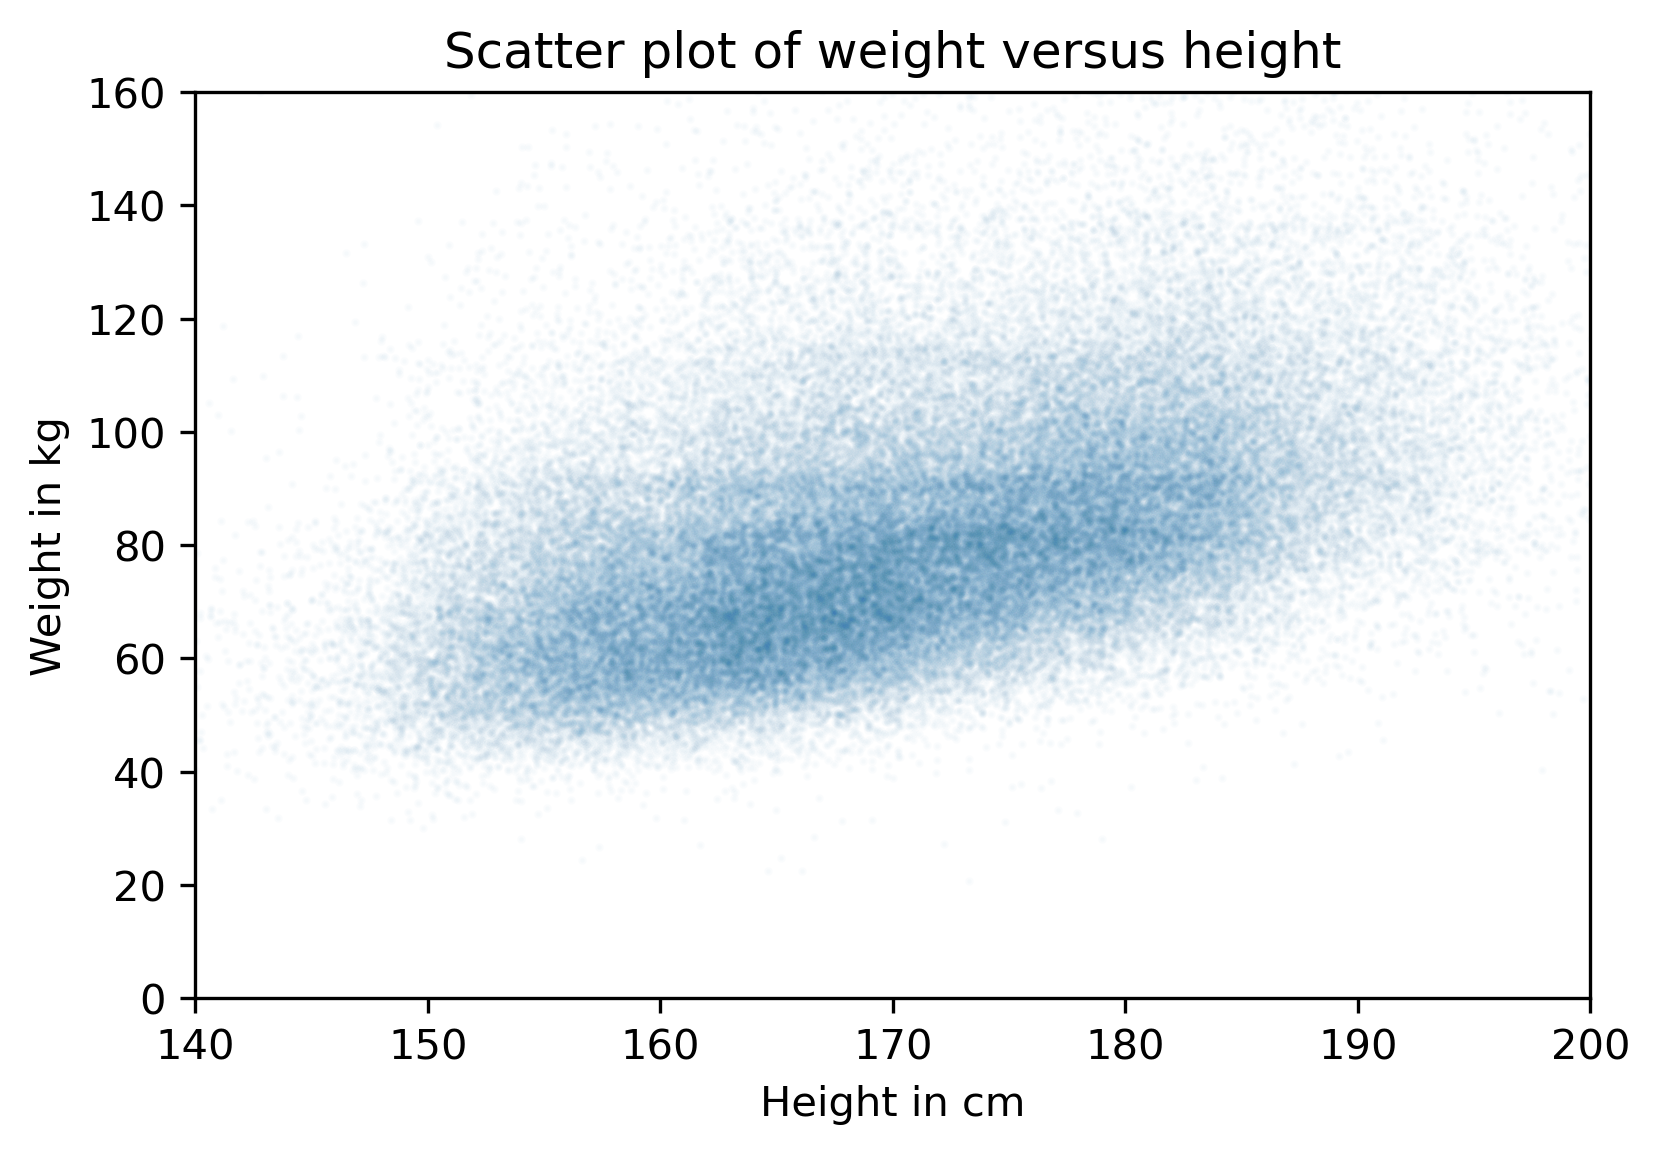
\includegraphics[scale=0.75]{09_relationships_files/09_relationships_26_0.png}
\end{center}

Now we have a reliable picture of the relationship between height and
weight.

Below you can see the misleading plot we started with and the more
reliable one we ended with. They are clearly different, and they suggest
different stories about the relationship between these variables.

\begin{lstlisting}[language=Python,style=source]
# Set the figure size
plt.figure(figsize=(8, 3))

# Create subplots with 2 rows, 1 column, and start plot 1
plt.subplot(1, 2, 1)
plt.plot(height, weight, 'o')

plt.xlabel('Height in cm')
plt.ylabel('Weight in kg')
plt.title('Scatter plot of weight versus height')

# Adjust the layout so the two plots don't overlap
plt.tight_layout()

# Start plot 2
plt.subplot(1, 2, 2)

plt.plot(height_jitter, weight_jitter, 'o', 
         alpha=0.02, markersize=1)

plt.xlim([140, 200])
plt.ylim([0, 160])
plt.xlabel('Height in cm')
plt.ylabel('Weight in kg')
plt.title('Scatter plot of weight versus height')
plt.tight_layout()
\end{lstlisting}

\begin{center}
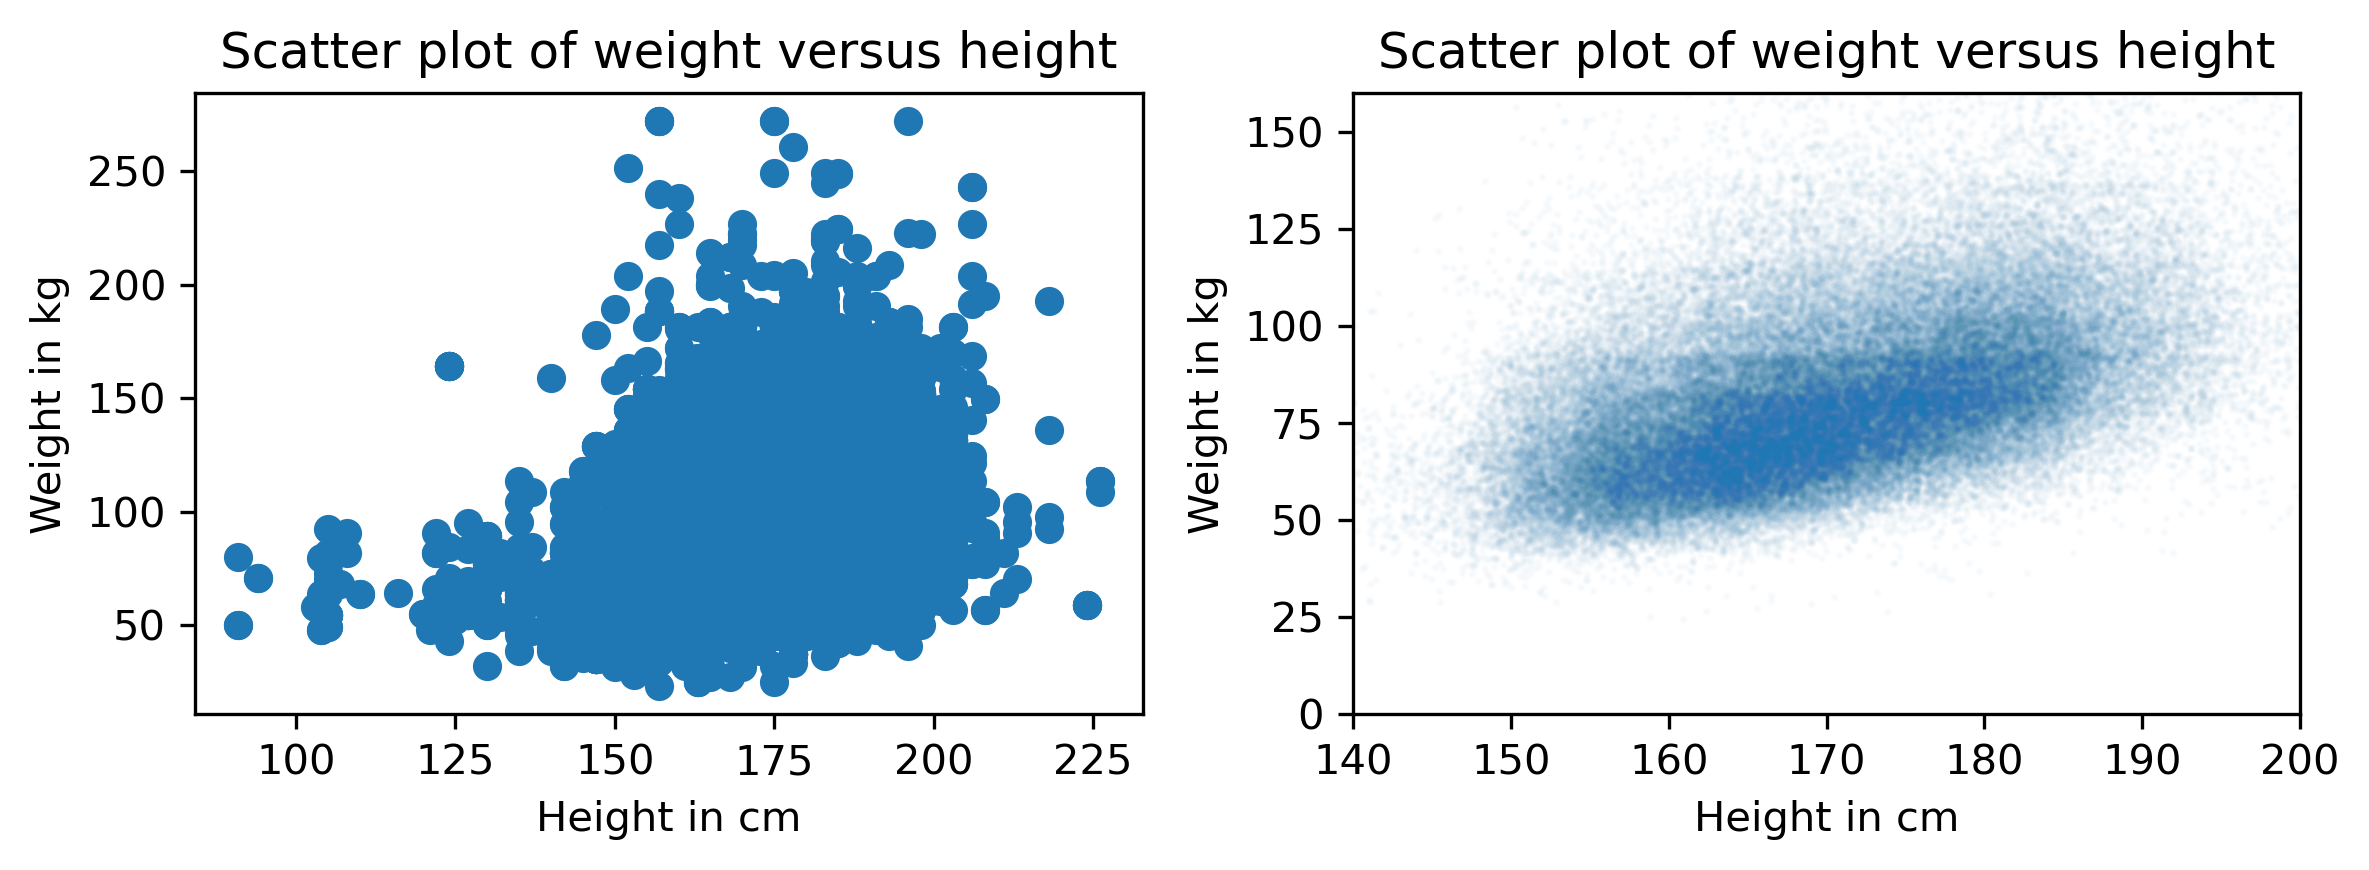
\includegraphics[scale=0.75]{09_relationships_files/09_relationships_28_0.png}
\end{center}

The point of this example is that it takes some effort to make an
effective scatter plot.

\textbf{Exercise:} Do people tend to gain weight as they get older? We
can answer this question by visualizing the relationship between weight
and age.

But before we make a scatter plot, it is a good idea to visualize
distributions one variable at a time. So let's look at the distribution
of age.

The BRFSS dataset includes a column, \passthrough{\lstinline!AGE!},
which represents each respondent's age in years. To protect respondents'
privacy, ages are rounded off into 5-year bins.
\passthrough{\lstinline!AGE!} contains the midpoint of the bins.

\begin{itemize}
\item
  Extract the variable \passthrough{\lstinline!'AGE'!} from the
  DataFrame \passthrough{\lstinline!brfss!} and assign it to
  \passthrough{\lstinline!age!}.
\item
  Plot the PMF of \passthrough{\lstinline!age!} as a bar chart, using
  \passthrough{\lstinline!Pmf!} from
  \passthrough{\lstinline!empiricaldist!}.
\end{itemize}

\begin{lstlisting}[language=Python,style=source]
from empiricaldist import Pmf
\end{lstlisting}

\textbf{Exercise:} Now let's look at the distribution of weight. The
column that contains weight in kilograms is
\passthrough{\lstinline!WTKG3!}. Because this column contains many
unique values, displaying it as a PMF doesn't work very well.

\begin{lstlisting}[language=Python,style=source]
Pmf.from_seq(weight).bar()

plt.xlabel('Weight in kg')
plt.ylabel('PMF')
plt.title('Distribution of weight');
\end{lstlisting}

\begin{center}
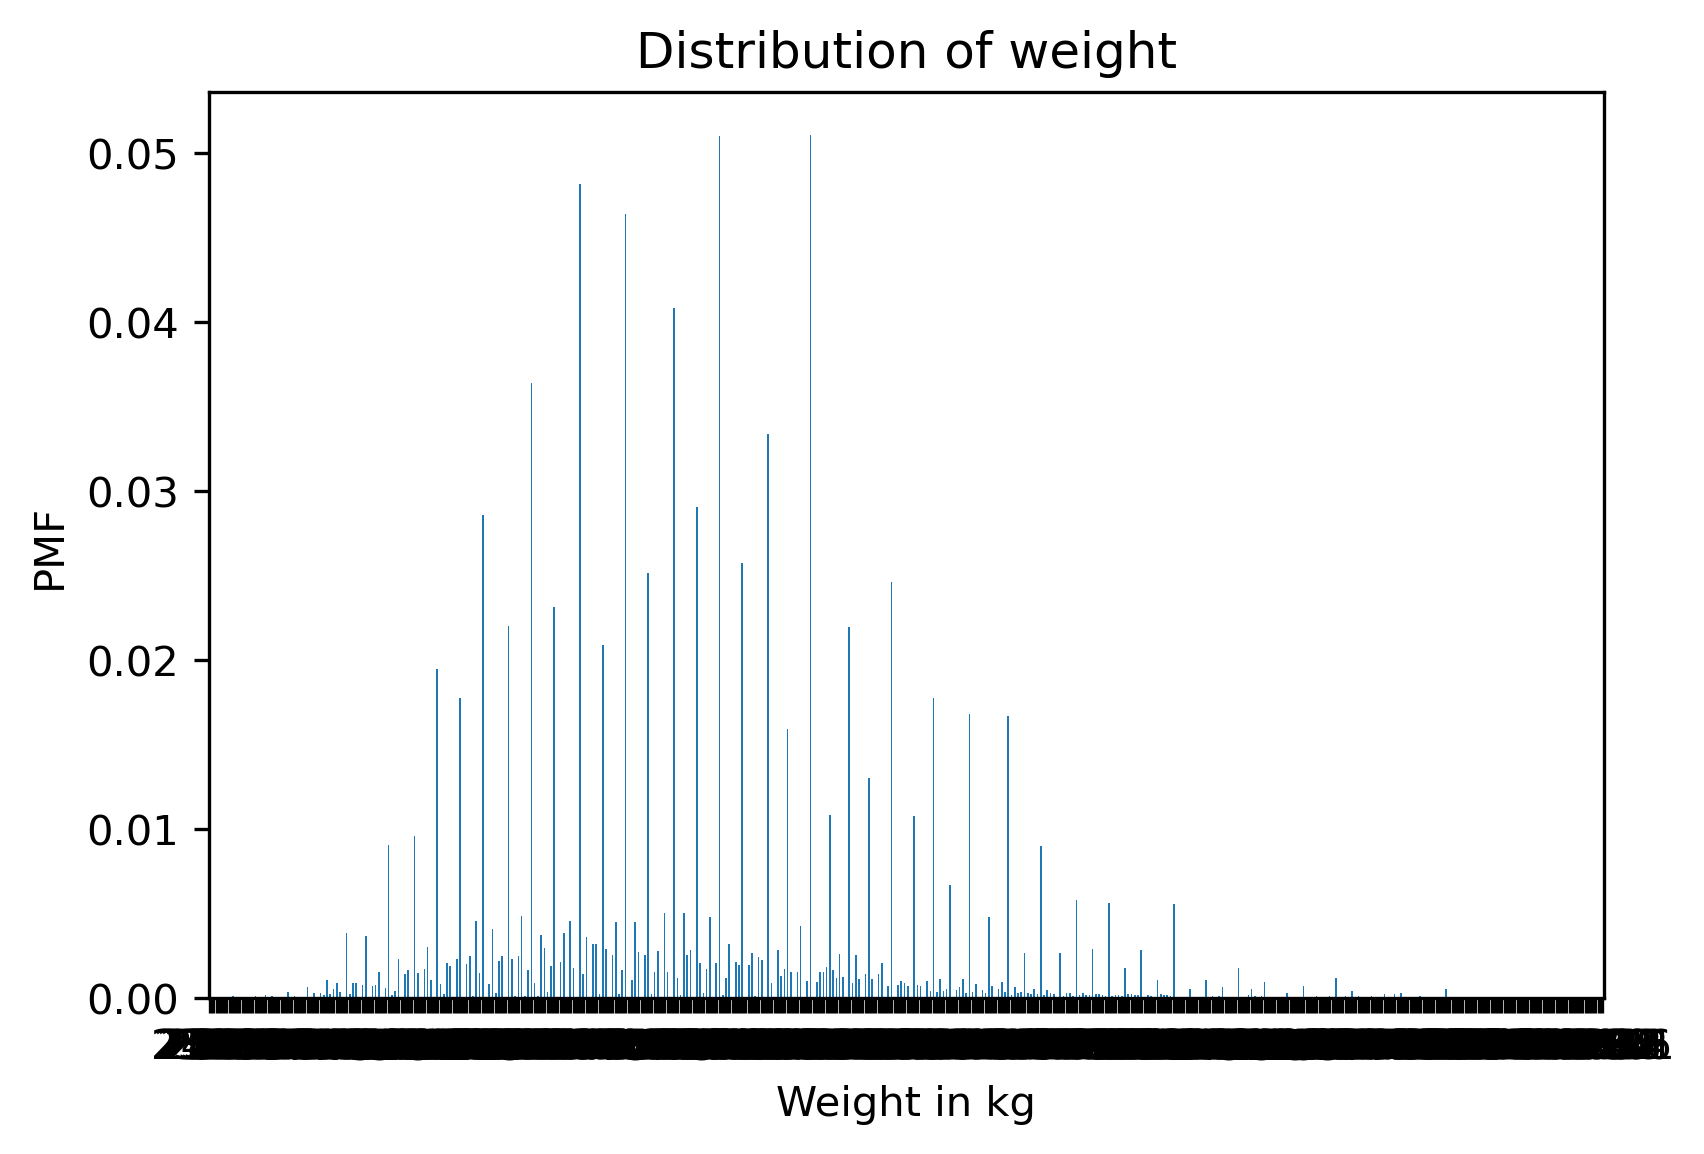
\includegraphics[scale=0.75]{09_relationships_files/09_relationships_34_0.png}
\end{center}

To get a better view of this distribution, try plotting the CDF.

Compute the CDF of a normal distribution with the same mean and standard
deviation, and compare it with the distribution of weight. Is the normal
distribution a good model for this data? What about log-transformed
weights?

\textbf{Exercise:} Now let's make a scatter plot of
\passthrough{\lstinline!weight!} versus \passthrough{\lstinline!age!}.
Adjust \passthrough{\lstinline!alpha!} and
\passthrough{\lstinline!markersize!} to avoid overplotting. Use
\passthrough{\lstinline!ylim!} to limit the \passthrough{\lstinline!y!}
axis from 0 to 200 kilograms.

\textbf{Exercise:} In the previous exercise, the ages fall in columns
because they've been rounded into 5-year bins. If we jitter them, the
scatter plot will show the relationship more clearly.

\begin{itemize}
\tightlist
\item
  Add random noise to \passthrough{\lstinline!age!} with mean
  \passthrough{\lstinline!0!} and standard deviation
  \passthrough{\lstinline!2.5!}.
\item
  Make a scatter plot and adjust \passthrough{\lstinline!alpha!} and
  \passthrough{\lstinline!markersize!} again.
\end{itemize}

\hypertarget{visualizing-relationships}{%
\section{Visualizing relationships}\label{visualizing-relationships}}

In the previous section we used scatter plots to visualize relationships
between variables, and in the exercises, you explored the relationship
between age and weight. In this section, we'll see other ways to
visualize these relationships, including boxplots and violin plots.

I'll start with a scatter plot of weight versus age.

\begin{lstlisting}[language=Python,style=source]
age = brfss['AGE']
noise = np.random.normal(0, 1.0, size=len(brfss))
age_jitter = age + noise

plt.plot(age_jitter, weight_jitter, 'o', 
         alpha=0.01, markersize=1)

plt.xlabel('Age in years')
plt.ylabel('Weight in kg')
plt.ylim([0, 200])
plt.title('Weight versus age');
\end{lstlisting}

\begin{center}
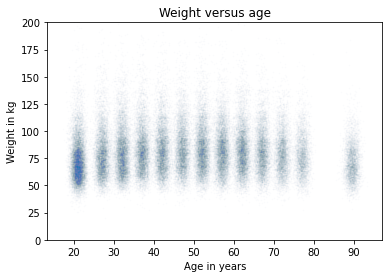
\includegraphics[scale=0.75]{09_relationships_files/09_relationships_39_0.png}
\end{center}

In this version of the scatter plot, I adjusted the jittering of the
weights so there's still space between the columns. That makes it
possible to see the shape of the distribution in each age group, and the
differences between groups. With this view, it looks like weight
increases until age 40 or 50, and then starts to decrease.

If we take this idea one step farther, we can use KDE to estimate the
density function in each column and plot it. And there's a name for
that; it's called a violin plot. Seaborn provides a function that makes
violin plots, but before we can use it, we have to get rid of any rows
with missing data. Here's how:

\begin{lstlisting}[language=Python,style=source]
data = brfss.dropna(subset=['AGE', 'WTKG3'])
data.shape
\end{lstlisting}

\begin{lstlisting}[style=output]
(92729, 9)
\end{lstlisting}

\passthrough{\lstinline!dropna()!} creates a new DataFrame that drops
the rows in \passthrough{\lstinline!brfss!} where
\passthrough{\lstinline!AGE!} or \passthrough{\lstinline!WTKG3!} are
\passthrough{\lstinline!NaN!}. Now we can call
\passthrough{\lstinline!violinplot!}.

\begin{lstlisting}[language=Python,style=source]
import seaborn as sns

sns.violinplot(x='AGE', y='WTKG3', data=data, inner=None)

plt.xlabel('Age in years')
plt.ylabel('Weight in kg')
plt.title('Weight versus age');
\end{lstlisting}

\begin{center}
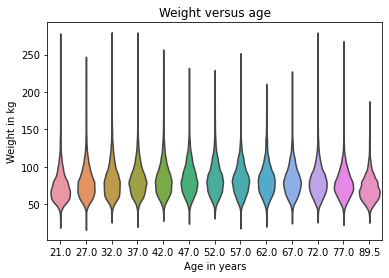
\includegraphics[scale=0.75]{09_relationships_files/09_relationships_43_0.png}
\end{center}

The \passthrough{\lstinline!x!} and \passthrough{\lstinline!y!}
arguments mean we want \passthrough{\lstinline!AGE!} on the x-axis and
\passthrough{\lstinline!WTKG3!} on the y-axis.
\passthrough{\lstinline!data!} is the DataFrame we just created, which
contains the variables we're going to plot. The argument
\passthrough{\lstinline!inner=None!} simplifies the plot a little.

In the figure, each shape represents the distribution of weight in one
age group. The width of these shapes is proportional to the estimated
density, so it's like two vertical KDEs plotted back to back (and filled
in with nice colors).

Another, related way to look at data like this is called a \textbf{box
plot}. The code to generate a box plot is very similar.

\begin{lstlisting}[language=Python,style=source]
sns.boxplot(x='AGE', y='WTKG3', data=data, whis=10)

plt.xlabel('Age in years')
plt.ylabel('Weight in kg')
plt.title('Weight versus age');
\end{lstlisting}

\begin{center}
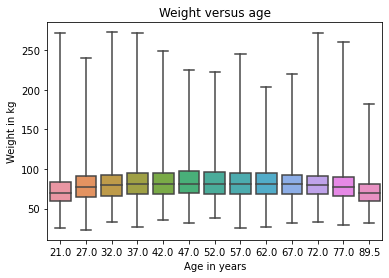
\includegraphics[scale=0.75]{09_relationships_files/09_relationships_45_0.png}
\end{center}

I included the argument \passthrough{\lstinline!whis=10!} to turn off a
feature we don't need. If you are curious about it, you can
\href{https://seaborn.pydata.org/generated/seaborn.boxplot.html}{read
the documentation}.

Each box represents the distribution of weight in an age group. The
height of each box represents the range from the 25th to the 75th
percentile. The line in the middle of each box is the median. The spines
sticking out of the top and bottom show the minimum and maximum values.

In my opinion, this plot gives us the best view of the relationship
between weight and age.

\begin{itemize}
\item
  Looking at the medians, it seems like people in their 40s are the
  heaviest; younger and older people are lighter.
\item
  Looking at the sizes of the boxes, it seems like people in their 40s
  have the most variability in weight, too.
\item
  These plots also show how skewed the distribution of weight is; that
  is, the heaviest people are much farther from the median than the
  lightest people.
\end{itemize}

For data that skews toward higher values, it is sometimes useful to look
at it on a logarithmic scale.

We can do that with the Pyplot function
\passthrough{\lstinline!yscale!}.

\begin{lstlisting}[language=Python,style=source]
sns.boxplot(x='AGE', y='WTKG3', data=data, whis=10)

plt.yscale('log')
plt.xlabel('Age in years')
plt.ylabel('Weight in kg (log scale)')
plt.title('Weight versus age');
\end{lstlisting}

\begin{center}
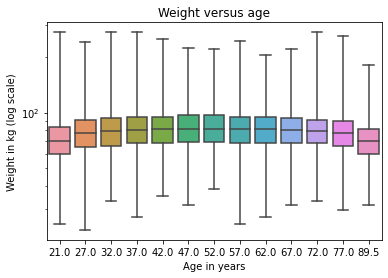
\includegraphics[scale=0.75]{09_relationships_files/09_relationships_47_0.png}
\end{center}

To show the relationship between age and weight most clearly, this is
probably the figure I would use.

In the following exercises, you'll have a chance to generate violin and
box plots for other variables.

\textbf{Exercise:} Previously we looked at a scatter plot of height and
weight, and saw that taller people tend to be heavier. Now let's take a
closer look using a box plot. The \passthrough{\lstinline!brfss!}
DataFrame contains a column named \passthrough{\lstinline!\_HTMG10!}
that represents height in centimeters, binned into 10 cm groups.

\begin{itemize}
\item
  Make a boxplot that shows the distribution of weight in each height
  group.
\item
  Plot the y-axis on a logarithmic scale.
\end{itemize}

Suggestion: If the labels on the \passthrough{\lstinline!x!} axis
collide, you can rotate them like this:

\begin{lstlisting}[style=output]
plt.xticks(rotation='45')
\end{lstlisting}

\textbf{Exercise:} As a second example, let's look at the relationship
between income and height.

In the BRFSS, income is represented as a categorical variable; that is,
respondents are assigned to one of 8 income categories. The column name
is \passthrough{\lstinline!INCOME2!}.

Before we connect income with anything else, let's look at the
distribution by computing the PMF.

\begin{itemize}
\item
  Extract \passthrough{\lstinline!INCOME2!} from
  \passthrough{\lstinline!brfss!} and assign it to
  \passthrough{\lstinline!income!}.
\item
  Plot the PMF of \passthrough{\lstinline!income!} as a bar chart.
\end{itemize}

Note: You will see that about a third of the respondents are in the
highest income group; ideally, it would be better if there were more
groups at the high end, but we'll work with what we have.

\textbf{Exercise:} Generate a violin plot that shows the distribution of
height in each income group. Can you see a relationship between these
variables?

\hypertarget{correlation}{%
\section{Correlation}\label{correlation}}

In the previous section, we visualized relationships between pairs of
variables. Now we'll learn about the \textbf{coefficient of
correlation}, which quantifies the strength of these relationships.

When people say ``correlation'' casually, they might mean any
relationship between two variables. In statistics, it usually means
Pearson's correlation coefficient, which is a number between
\passthrough{\lstinline!-1!} and \passthrough{\lstinline!1!} that
quantifies the strength of a linear relationship between variables.

To demonstrate, I'll select three columns from the BRFSS dataset:

\begin{lstlisting}[language=Python,style=source]
columns = ['HTM4', 'WTKG3', 'AGE']
subset = brfss[columns]
\end{lstlisting}

The result is a DataFrame with just those columns. With this subset of
the data, we can use the \passthrough{\lstinline!corr!} method, like
this:

\begin{lstlisting}[language=Python,style=source]
subset.corr()
\end{lstlisting}

\begin{tabular}{lrrr}
\toprule
{} &      HTM4 &     WTKG3 &       AGE \\
\midrule
HTM4  &  1.000000 &  0.474203 & -0.093684 \\
WTKG3 &  0.474203 &  1.000000 &  0.021641 \\
AGE   & -0.093684 &  0.021641 &  1.000000 \\
\bottomrule
\end{tabular}

The result is a \textbf{correlation matrix}. Reading across the first
row, the correlation of \passthrough{\lstinline!HTM4!} with itself is
\passthrough{\lstinline!1!}. That's expected; the correlation of
anything with itself is \passthrough{\lstinline!1!}.

The next entry is more interesting; the correlation of height and weight
is about \passthrough{\lstinline!0.47!}. It's positive, which means
taller people are heavier, and it is moderate in strength, which means
it has some predictive value. If you know someone's height, you can make
a better guess about their weight, and vice versa.

The correlation between height and age is about
\passthrough{\lstinline!-0.09!}. It's negative, which means that older
people tend to be shorter, but it's weak, which means that knowing
someone's age would not help much if you were trying to guess their
height.

The correlation between age and weight is even smaller. It is tempting
to conclude that there is no relationship between age and weight, but we
have already seen that there is. So why is the correlation so low?
Remember that the relationship between weight and age looks like this.

\begin{lstlisting}[language=Python,style=source]
data = brfss.dropna(subset=['AGE', 'WTKG3'])
sns.boxplot(x='AGE', y='WTKG3', data=data, whis=10)

plt.xlabel('Age in years')
plt.ylabel('Weight in kg')
plt.title('Weight versus age');
\end{lstlisting}

\begin{center}
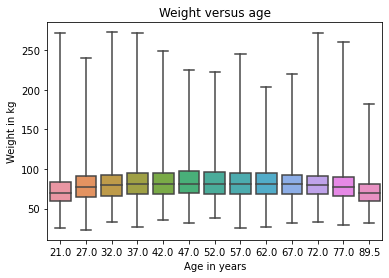
\includegraphics[scale=0.75]{09_relationships_files/09_relationships_58_0.png}
\end{center}

People in their forties are the heaviest; younger and older people are
lighter. So this relationship is nonlinear. But correlation only
measures linear relationships. If the relationship is nonlinear,
correlation generally underestimates how strong it is.

To demonstrate, I'll generate some fake data:
\passthrough{\lstinline!xs!} contains equally-spaced points between
\passthrough{\lstinline!-1!} and \passthrough{\lstinline!1!}.
\passthrough{\lstinline!ys!} is \passthrough{\lstinline!xs!} squared
plus some random noise.

\begin{lstlisting}[language=Python,style=source]
xs = np.linspace(-1, 1)
ys = xs**2 + np.random.normal(0, 0.05, len(xs))
\end{lstlisting}

Here's the scatter plot of \passthrough{\lstinline!xs!} and
\passthrough{\lstinline!ys!}.

\begin{lstlisting}[language=Python,style=source]
plt.plot(xs, ys, 'o', alpha=0.5)
plt.xlabel('x')
plt.ylabel('y')
plt.title('Scatter plot of a fake dataset');
\end{lstlisting}

\begin{center}
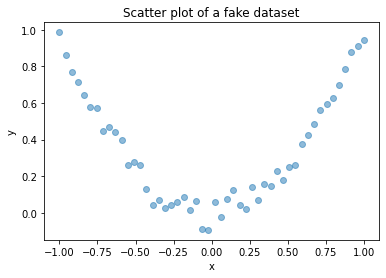
\includegraphics[scale=0.75]{09_relationships_files/09_relationships_62_0.png}
\end{center}

It's clear that this is a strong relationship; if you are given
\passthrough{\lstinline!x!}, you can make a much better guess about
\passthrough{\lstinline!y!}. But here's the correlation matrix:

\begin{lstlisting}[language=Python,style=source]
np.corrcoef(xs, ys)
\end{lstlisting}

\begin{lstlisting}[style=output]
array([[ 1.        , -0.02074742],
       [-0.02074742,  1.        ]])
\end{lstlisting}

Even though there is a strong non-linear relationship, the computed
correlation is close to \passthrough{\lstinline!0!}.

In general, if correlation is high -- that is, close to
\passthrough{\lstinline!1!} or \passthrough{\lstinline!-1!}, you can
conclude that there is a strong linear relationship. But if correlation
is close to \passthrough{\lstinline!0!}, that doesn't mean there is no
relationship; there might be a non-linear relationship.

This is one of the reasons I think correlation is not such a great
statistic. There's another reason to be careful with correlation; it
doesn't mean what people take it to mean. Specifically, correlation says
nothing about slope. If we say that two variables are correlated, that
means we can use one to predict the other. But that might not be what we
care about.

For example, suppose we are concerned about the health effects of weight
gain, so we plot weight versus age from 20 to 50 years old. I'll
generate two fake datasets to demonstrate the point. In each dataset,
\passthrough{\lstinline!xs!} represents age and
\passthrough{\lstinline!ys!} represents weight.

\begin{lstlisting}[language=Python,style=source]
np.random.seed(18)
xs1 = np.linspace(20, 50)
ys1 = 75 + 0.02 * xs1 + np.random.normal(0, 0.15, len(xs1))

plt.plot(xs1, ys1, 'o', alpha=0.5)
plt.xlabel('Age in years')
plt.ylabel('Weight in kg')
plt.title('Fake dataset #1');
\end{lstlisting}

\begin{center}
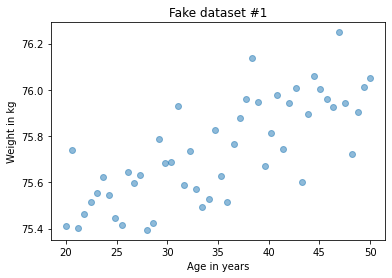
\includegraphics[scale=0.75]{09_relationships_files/09_relationships_67_0.png}
\end{center}

And here's the second dataset:

\begin{lstlisting}[language=Python,style=source]
np.random.seed(18)
xs2 = np.linspace(20, 50)
ys2 = 65 + 0.2 * xs2 + np.random.normal(0, 3, len(xs2))

plt.plot(xs2, ys2, 'o', alpha=0.5)
plt.xlabel('Age in years')
plt.ylabel('Weight in kg')
plt.title('Fake dataset #2');
\end{lstlisting}

\begin{center}
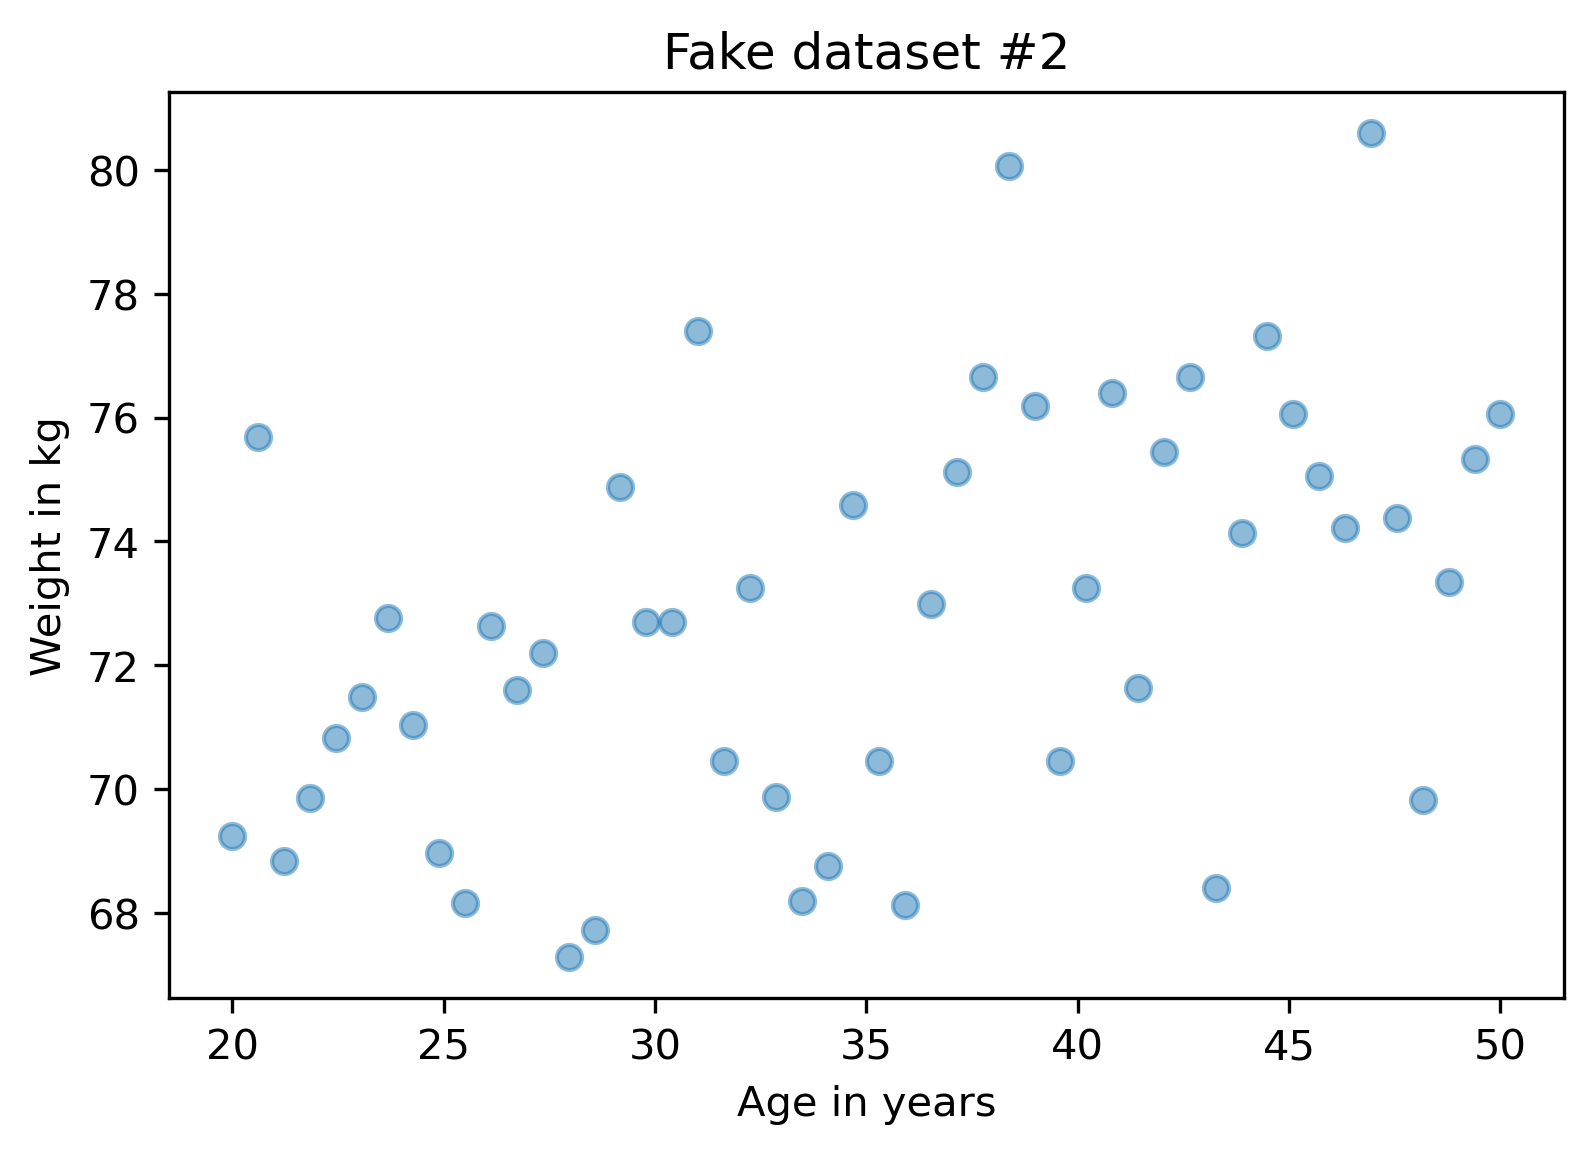
\includegraphics[scale=0.75]{09_relationships_files/09_relationships_69_0.png}
\end{center}

I constructed these examples so they look similar, but they have
substantially different correlations:

\begin{lstlisting}[language=Python,style=source]
rho1 = np.corrcoef(xs1, ys1)[0][1]
rho1
\end{lstlisting}

\begin{lstlisting}[style=output]
0.7579660563439401
\end{lstlisting}

\begin{lstlisting}[language=Python,style=source]
rho2 = np.corrcoef(xs2, ys2)[0][1]
rho2
\end{lstlisting}

\begin{lstlisting}[style=output]
0.4782776976576317
\end{lstlisting}

In the first example, the correlation is strong, close to
\passthrough{\lstinline!0.75!}. In the second example, the correlation
is moderate, close to \passthrough{\lstinline!0.5!}. So we might think
the first relationship is more important. But look more closely at the
\passthrough{\lstinline!y!} axis in both figures.

In the first example, the average weight gain over 30 years is less than
1 kilogram; in the second it is more than 5 kilograms! If we are
concerned about the health effects of weight gain, the second
relationship is probably more important, even though the correlation is
lower.\\
The statistic we really care about is the slope of the line, not the
coefficient of correlation.

In the next section, we'll see how to estimate that slope. But first,
let's practice with correlation.

\textbf{Exercise:} The purpose of the BRFSS is to explore health risk
factors, so it includes questions about diet. The column
\passthrough{\lstinline!\_VEGESU1!} represents the number of servings of
vegetables respondents reported eating per day.

Let's see how this variable relates to age and income.

\begin{itemize}
\tightlist
\item
  From the \passthrough{\lstinline!brfss!} DataFrame, select the columns
  \passthrough{\lstinline!'AGE'!}, \passthrough{\lstinline!INCOME2!},
  and \passthrough{\lstinline!\_VEGESU1!}.
\item
  Compute the correlation matrix for these variables.
\end{itemize}

\textbf{Exercise:} In the previous exercise, the correlation between
income and vegetable consumption is about
\passthrough{\lstinline!0.12!}. The correlation between age and
vegetable consumption is about \passthrough{\lstinline!-0.01!}.

Which of the following are correct interpretations of these results?

\begin{itemize}
\tightlist
\item
  \emph{A}: People in this dataset with higher incomes eat more
  vegetables.
\item
  \emph{B}: The relationship between income and vegetable consumption is
  linear.
\item
  \emph{C}: Older people eat more vegetables.
\item
  \emph{D}: There could be a strong non-linear relationship between age
  and vegetable consumption.
\end{itemize}

\textbf{Exercise:} In general it is a good idea to visualize the
relationship between variables \emph{before} you compute a correlation.
We didn't do that in the previous example, but it's not too late.

Generate a visualization of the relationship between age and vegetables.
How would you describe the relationship, if any?

\hypertarget{simple-regression}{%
\section{Simple regression}\label{simple-regression}}

In the previous section we saw that correlation does not always measure
what we really want to know. In this section, we look at an alternative:
simple linear regression.

Let's look again at the relationship between weight and age. In the
previous section, I generated two fake datasets to make a point:

\begin{lstlisting}[language=Python,style=source]
plt.figure(figsize=(8, 3))

plt.subplot(1, 2, 1)
plt.plot(xs1, ys1, 'o', alpha=0.5)
plt.xlabel('Age in years')
plt.ylabel('Weight in kg')
plt.title('Fake dataset #1')
plt.tight_layout()

plt.subplot(1, 2, 2)
plt.plot(xs2, ys2, 'o', alpha=0.5)
plt.xlabel('Age in years')
plt.ylabel('Weight in kg')
plt.title('Fake dataset #2')
plt.tight_layout()
\end{lstlisting}

\begin{center}
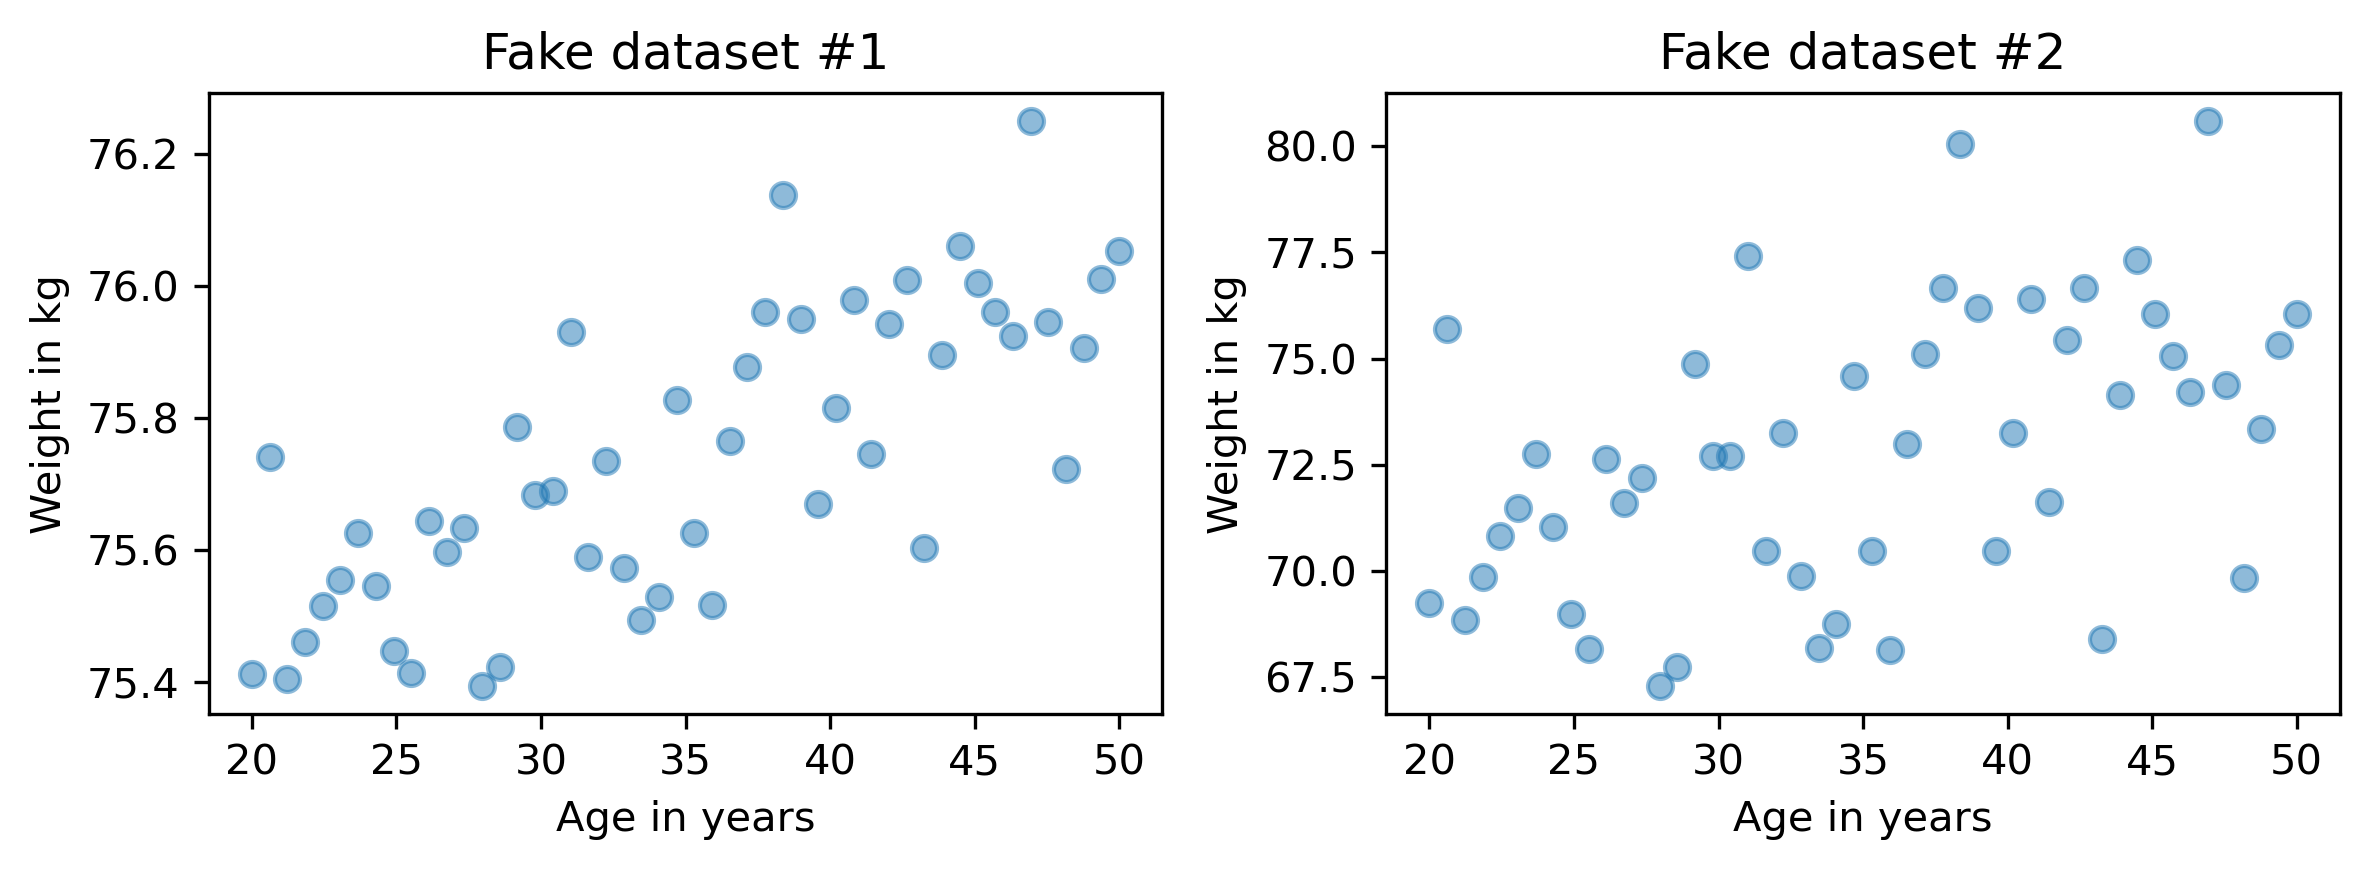
\includegraphics[scale=0.75]{09_relationships_files/09_relationships_78_0.png}
\end{center}

The one on the left has higher correlation, about 0.75 compared to 0.5.
But in this context, the statistic we probably care about is the slope
of the line, not the correlation coefficient. To estimate the slope, we
can use \passthrough{\lstinline!linregress!} from the SciPy
\passthrough{\lstinline!stats!} library.

\begin{lstlisting}[language=Python,style=source]
from scipy.stats import linregress

res1 = linregress(xs1, ys1)
res1._asdict()
\end{lstlisting}

\begin{lstlisting}[style=output]
{'slope': 0.018821034903244386,
 'intercept': 75.08049023710964,
 'rvalue': 0.7579660563439402,
 'pvalue': 1.8470158725246148e-10,
 'stderr': 0.002337849260560818,
 'intercept_stderr': 0.08439154079040358}
\end{lstlisting}

The result is a \passthrough{\lstinline!LinregressResult!} object that
contains five values: \passthrough{\lstinline!slope!} is the slope of
the line of best fit for the data; \passthrough{\lstinline!intercept!}
is the intercept.

For Fake Dataset \#1, the estimated slope is about 0.019 kilograms per
year or about 0.56 kilograms over the 30-year range.

\begin{lstlisting}[language=Python,style=source]
res1.slope * 30
\end{lstlisting}

\begin{lstlisting}[style=output]
0.5646310470973316
\end{lstlisting}

Here are the results for Fake Dataset \#2.

\begin{lstlisting}[language=Python,style=source]
res2 = linregress(xs2, ys2)
res2._asdict()
\end{lstlisting}

\begin{lstlisting}[style=output]
{'slope': 0.17642069806488855,
 'intercept': 66.60980474219305,
 'rvalue': 0.47827769765763173,
 'pvalue': 0.0004430600283776241,
 'stderr': 0.04675698521121631,
 'intercept_stderr': 1.6878308158080697}
\end{lstlisting}

The estimated slope is almost 10 times higher: about 0.18 kilograms per
year or about 5.3 kilograms per 30 years:

\begin{lstlisting}[language=Python,style=source]
res2.slope * 30
\end{lstlisting}

\begin{lstlisting}[style=output]
5.292620941946657
\end{lstlisting}

What's called \passthrough{\lstinline!rvalue!} here is correlation,
which confirms what we saw before; the first example has higher
correlation, about 0.75 compared to 0.5. But the strength of the effect,
as measured by the slope of the line, is about 10 times higher in the
second example.

We can use the results from \passthrough{\lstinline!linregress!} to
compute the line of best fit: first we get the minimum and maximum of
the observed \passthrough{\lstinline!xs!}; then we multiply by the slope
and add the intercept. Here's what that looks like for the first
example.

\begin{lstlisting}[language=Python,style=source]
plt.plot(xs1, ys1, 'o', alpha=0.5)

fx = np.array([xs1.min(), xs1.max()])
fy = res1.intercept + res1.slope * fx
plt.plot(fx, fy, '-')

plt.xlabel('Age in years')
plt.ylabel('Weight in kg')
plt.title('Fake Dataset #1');
\end{lstlisting}

\begin{center}
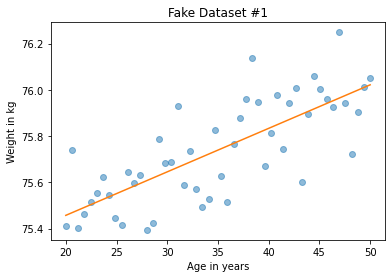
\includegraphics[scale=0.75]{09_relationships_files/09_relationships_88_0.png}
\end{center}

And the same thing for the second example.

\begin{lstlisting}[language=Python,style=source]
plt.plot(xs2, ys2, 'o', alpha=0.5)

fx = np.array([xs2.min(), xs2.max()])
fy = res2.intercept + res2.slope * fx
plt.plot(fx, fy, '-')

plt.xlabel('Age in years')
plt.ylabel('Weight in kg')
plt.title('Fake Dataset #2');
\end{lstlisting}

\begin{center}
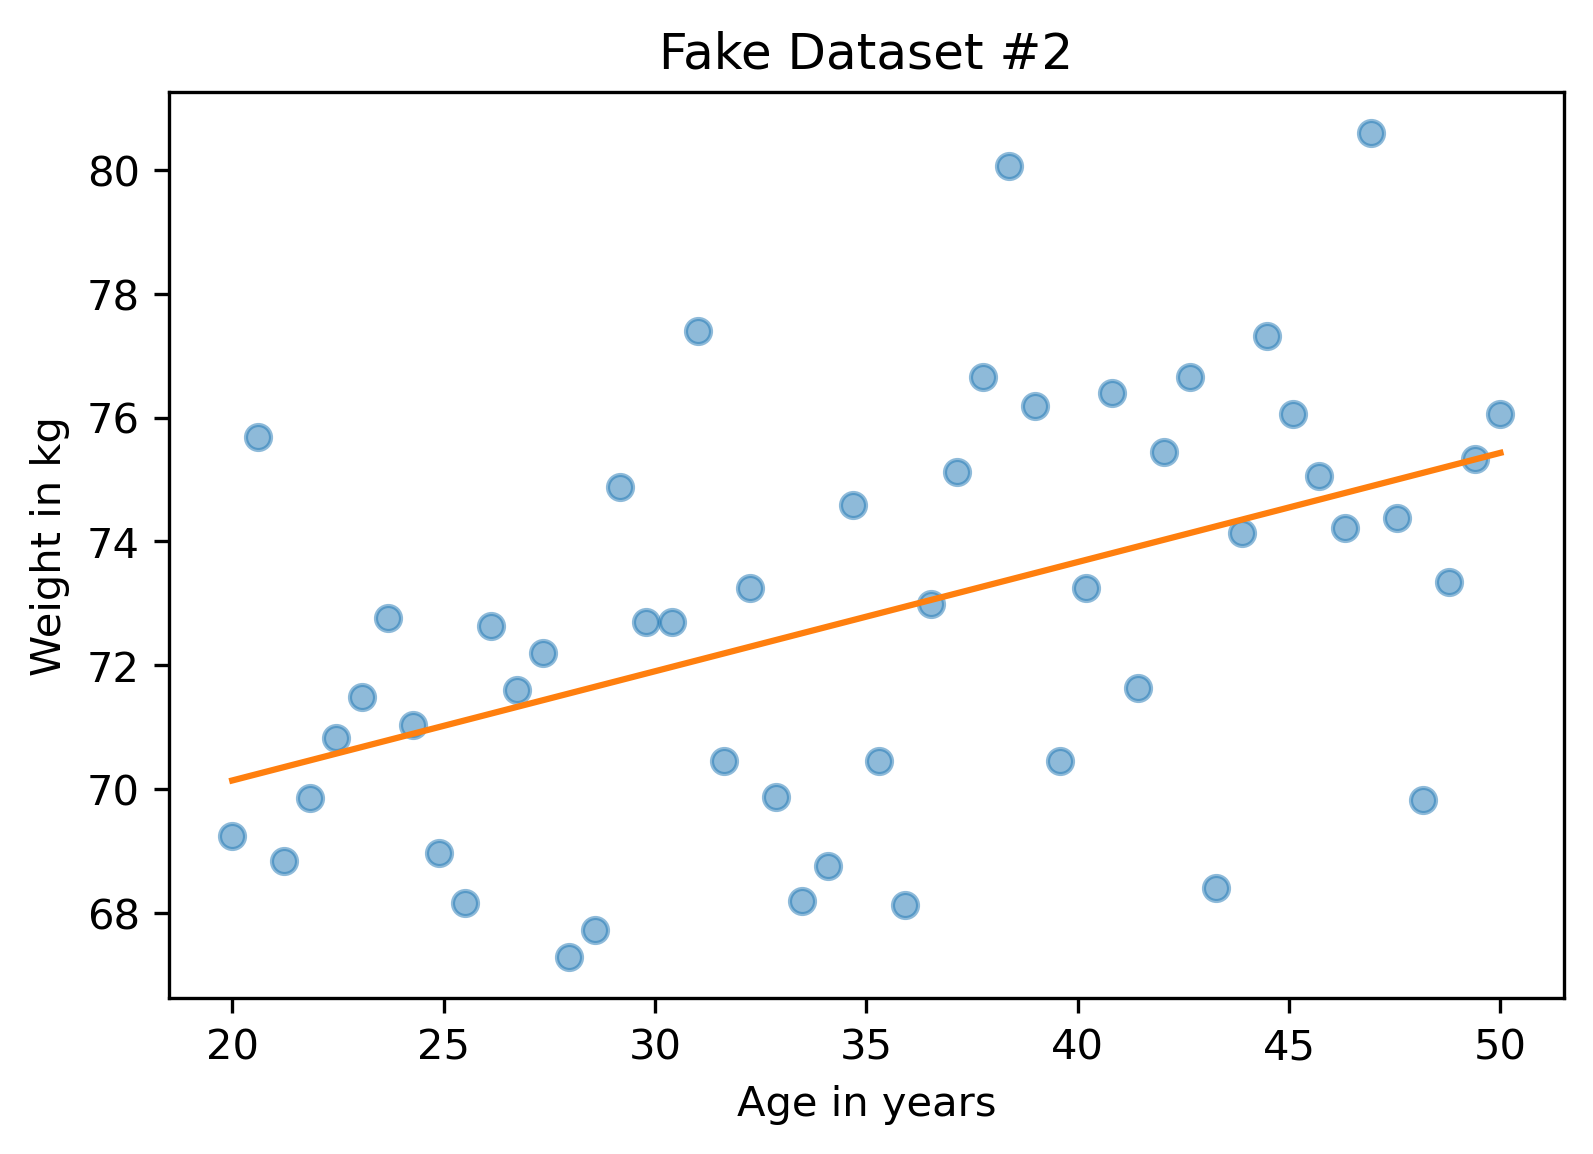
\includegraphics[scale=0.75]{09_relationships_files/09_relationships_90_0.png}
\end{center}

The visualization here might be misleading unless you look closely at
the vertical scales; the slope in the second figure is almost 10 times
higher.

\hypertarget{height-and-weight}{%
\section{Height and weight}\label{height-and-weight}}

Now let's look at an example with real data. Here's the scatter plot of
height and weight one more time.

\begin{lstlisting}[language=Python,style=source]
plt.plot(height_jitter, weight_jitter, 'o', 
         alpha=0.02, markersize=1)

plt.xlim([140, 200])
plt.ylim([0, 160])
plt.xlabel('Height in cm')
plt.ylabel('Weight in kg')
plt.title('Scatter plot of weight versus height');
\end{lstlisting}

\begin{center}
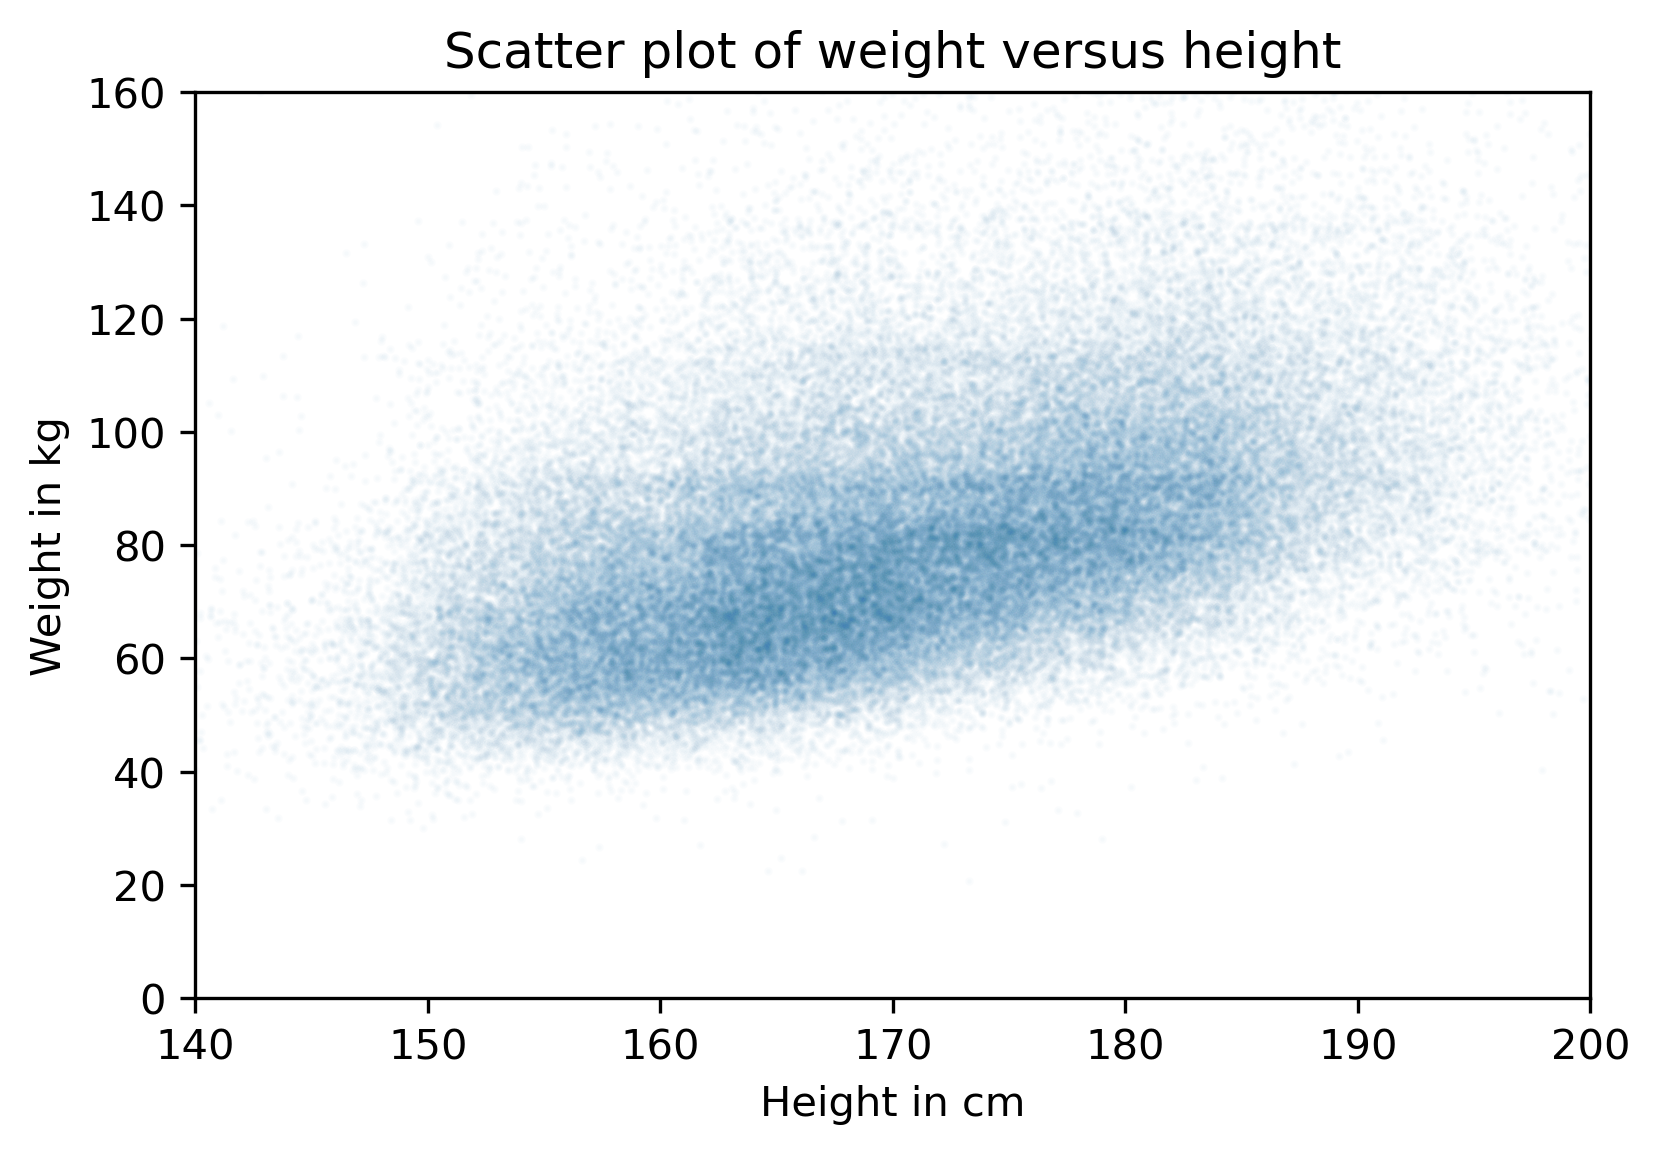
\includegraphics[scale=0.75]{09_relationships_files/09_relationships_93_0.png}
\end{center}

Now we can compute the regression line.
\passthrough{\lstinline!linregress!} can't handle
\passthrough{\lstinline!NaN!}, so we have to use
\passthrough{\lstinline!dropna!} to remove rows that are missing the
data we need.

\begin{lstlisting}[language=Python,style=source]
subset = brfss.dropna(subset=['WTKG3', 'HTM4'])
height_clean = subset['HTM4']
weight_clean = subset['WTKG3']
\end{lstlisting}

Now we can compute the linear regression.

\begin{lstlisting}[language=Python,style=source]
res_hw = linregress(height_clean, weight_clean)
res_hw._asdict()
\end{lstlisting}

\begin{lstlisting}[style=output]
{'slope': 0.9192115381848297,
 'intercept': -75.12704250330233,
 'rvalue': 0.47420308979024584,
 'pvalue': 0.0,
 'stderr': 0.005632863769802998,
 'intercept_stderr': 0.9608860265433182}
\end{lstlisting}

The slope is about 0.92 kilograms per centimeter, which means that we
expect a person one centimeter taller to be almost a kilogram heavier.
That's quite a lot.

As before, we can compute the line of best fit:

\begin{lstlisting}[language=Python,style=source]
fx = np.array([height_clean.min(), height_clean.max()])
fy = res_hw.intercept + res_hw.slope * fx
\end{lstlisting}

And here's what that looks like.

\begin{lstlisting}[language=Python,style=source]
plt.plot(height_jitter, weight_jitter, 'o', alpha=0.02, markersize=1)

plt.plot(fx, fy, '-')

plt.xlim([140, 200])
plt.ylim([0, 160])
plt.xlabel('Height in cm')
plt.ylabel('Weight in kg')
plt.title('Scatter plot of weight versus height');
\end{lstlisting}

\begin{center}
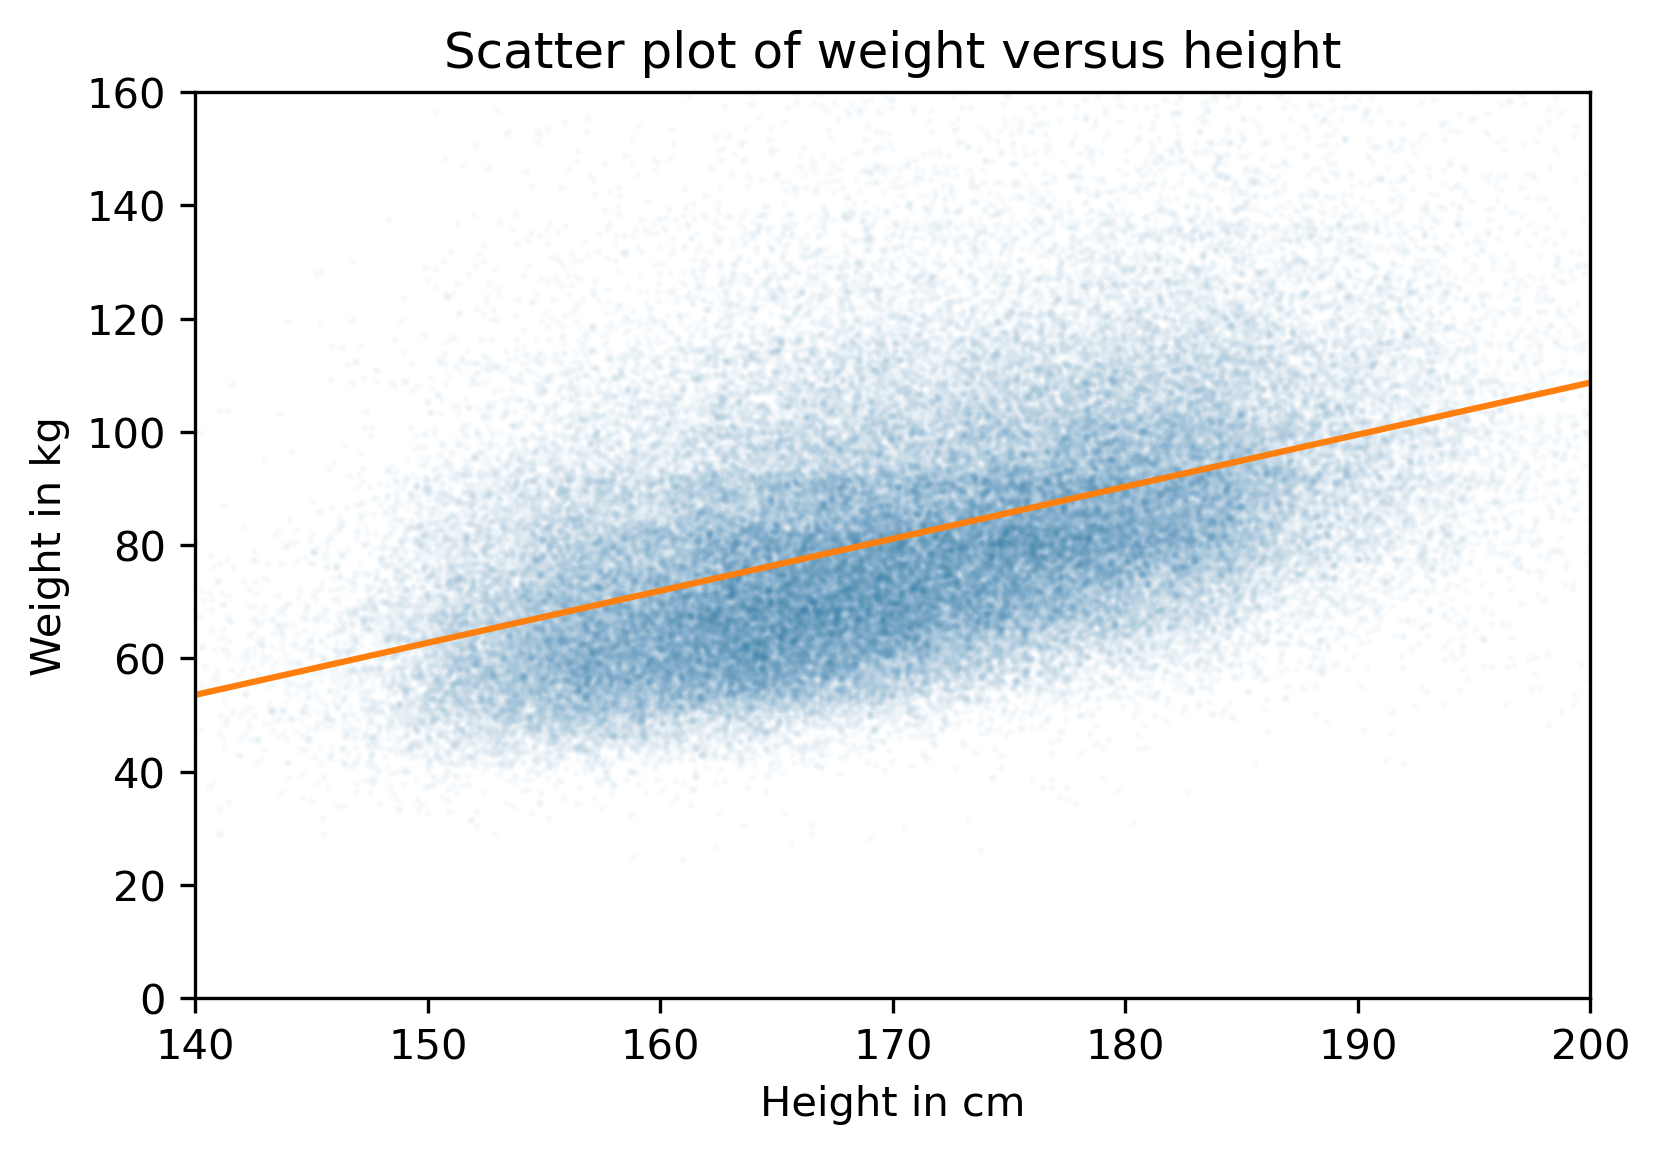
\includegraphics[scale=0.75]{09_relationships_files/09_relationships_101_0.png}
\end{center}

The slope of this line seems consistent with the scatter plot.

Linear regression has the same problem as correlation; it only measures
the strength of a linear relationship. Here's the scatter plot of weight
versus age, which we saw earlier.

\begin{lstlisting}[language=Python,style=source]
plt.plot(age_jitter, weight_jitter, 'o', 
         alpha=0.01, markersize=1)

plt.ylim([0, 160])
plt.xlabel('Age in years')
plt.ylabel('Weight in kg')
plt.title('Weight versus age');
\end{lstlisting}

\begin{center}
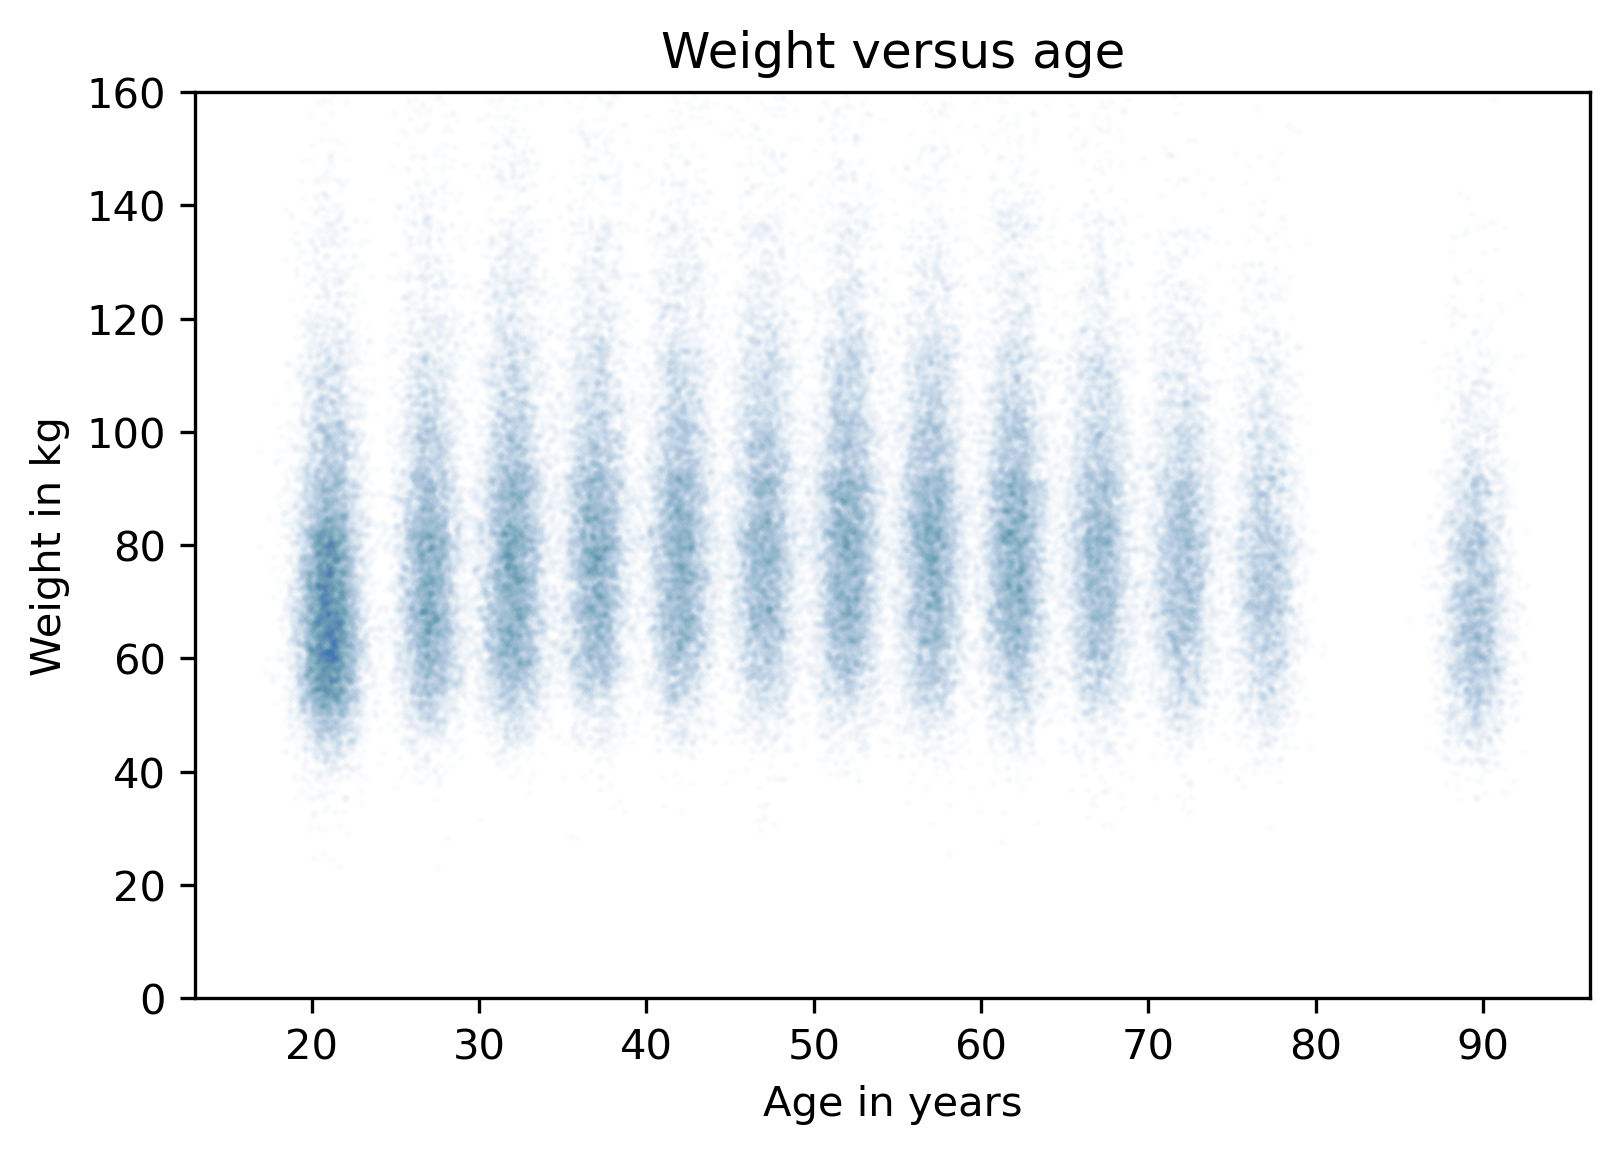
\includegraphics[scale=0.75]{09_relationships_files/09_relationships_103_0.png}
\end{center}

People in their 40s are the heaviest; younger and older people are
lighter. So the relationship is nonlinear.

If we don't look at the scatter plot and blindly compute the regression
line, here's what we get.

\begin{lstlisting}[language=Python,style=source]
subset = brfss.dropna(subset=['WTKG3', 'AGE'])
age_clean = subset['AGE']
weight_clean = subset['WTKG3']

res_aw = linregress(age_clean, weight_clean)
res_aw._asdict()
\end{lstlisting}

\begin{lstlisting}[style=output]
{'slope': 0.023981159566968724,
 'intercept': 80.07977583683224,
 'rvalue': 0.021641432889064068,
 'pvalue': 4.374327493007566e-11,
 'stderr': 0.003638139410742186,
 'intercept_stderr': 0.18688508176870167}
\end{lstlisting}

The estimated slope is only 0.02 kilograms per year, or 0.6 kilograms in
30 years. And here's what the line of best fit looks like.

\begin{lstlisting}[language=Python,style=source]
plt.plot(age_jitter, weight_jitter, 'o', 
         alpha=0.01, markersize=1)

fx = np.array([age_clean.min(), age_clean.max()])
fy = res_aw.intercept + res_aw.slope * fx
plt.plot(fx, fy, '-')

plt.ylim([0, 160])
plt.xlabel('Age in years')
plt.ylabel('Weight in kg')
plt.title('Weight versus age');
\end{lstlisting}

\begin{center}
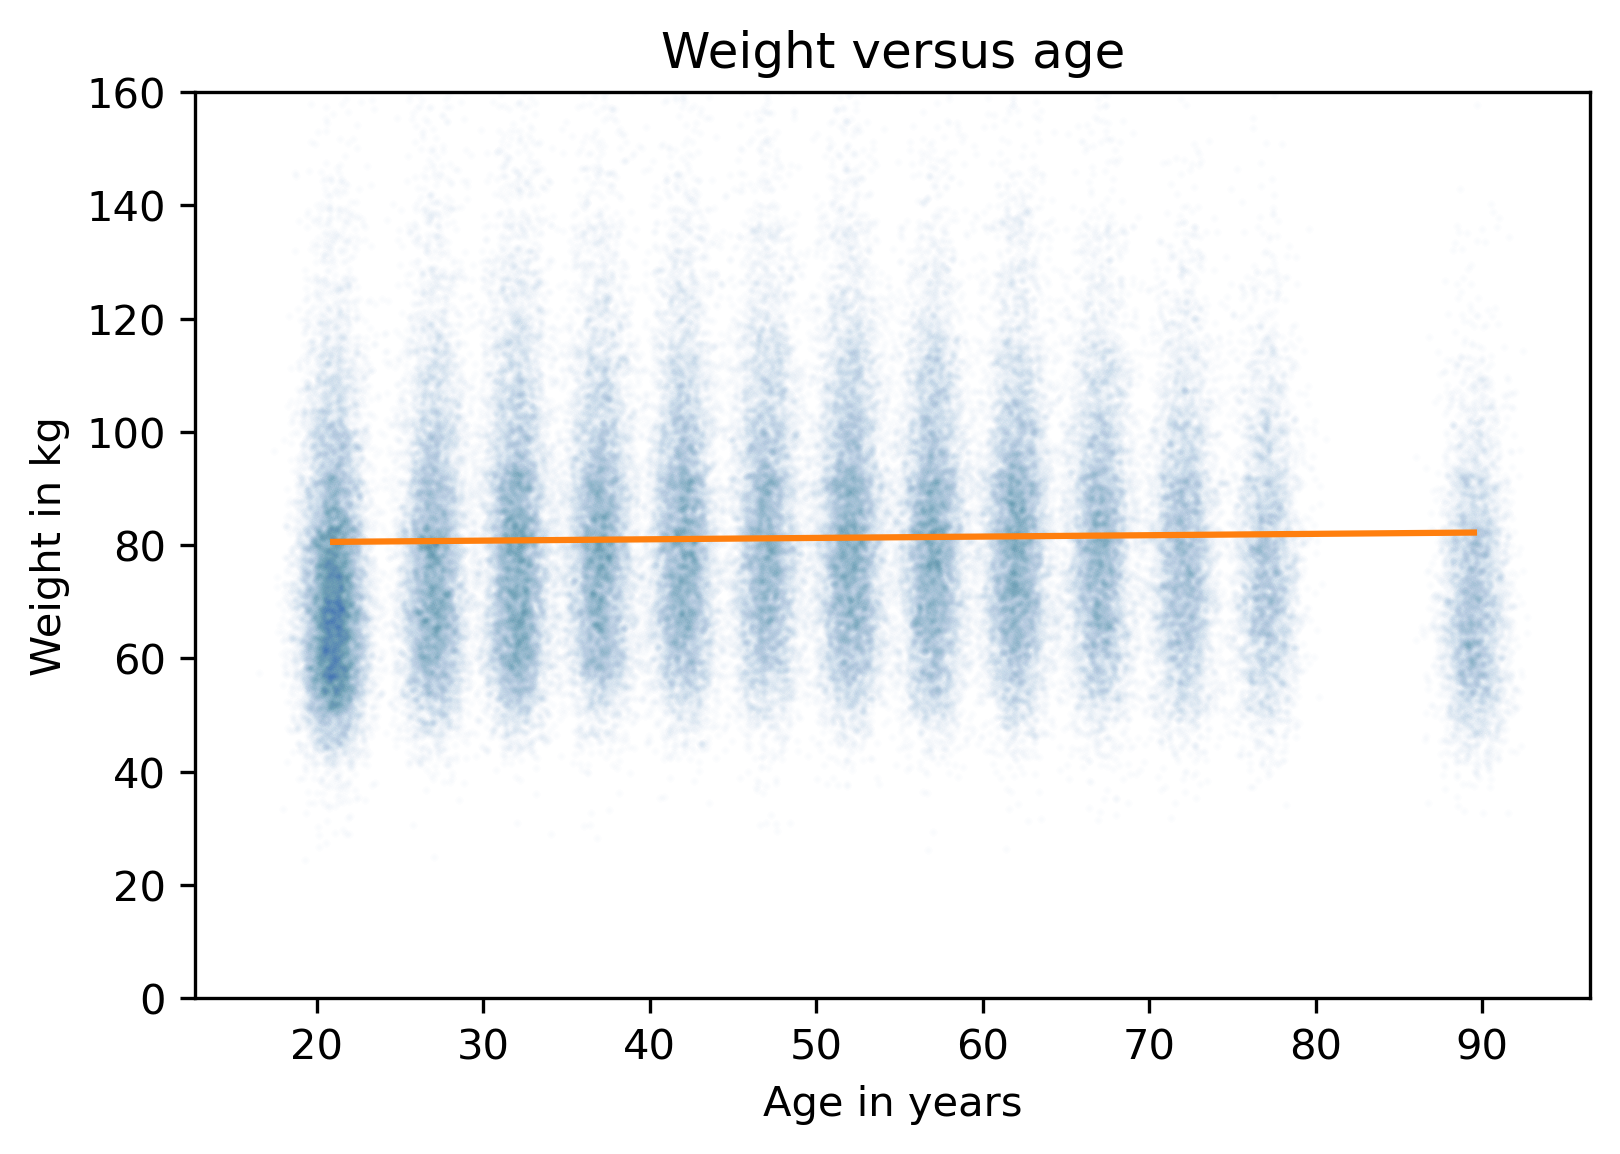
\includegraphics[scale=0.75]{09_relationships_files/09_relationships_107_0.png}
\end{center}

A straight line does not capture the relationship between these
variables well.

In the next chapter, you'll see how to use multiple regression to
estimate non-linear relationships. But first, let's practice simple
regression.

\textbf{Exercise:} Who do you think eats more vegetables, people with
low income, or people with high income? Let's find out.

As we've seen previously, the column \passthrough{\lstinline!INCOME2!}
represents income level and \passthrough{\lstinline!\_VEGESU1!}
represents the number of vegetable servings respondents reported eating
per day.

Make a scatter plot with vegetable servings versus income, that is, with
vegetable servings on the \passthrough{\lstinline!y!} axis and income
group on the \passthrough{\lstinline!x!} axis.

You might want to use \passthrough{\lstinline!ylim!} to zoom in on the
bottom half of the \passthrough{\lstinline!y!} axis.

\textbf{Exercise:} Now let's estimate the slope of the relationship
between vegetable consumption and income.

\begin{itemize}
\item
  Use \passthrough{\lstinline!dropna!} to select rows where
  \passthrough{\lstinline!INCOME2!} and
  \passthrough{\lstinline!\_VEGESU1!} are not
  \passthrough{\lstinline!NaN!}.
\item
  Extract \passthrough{\lstinline!INCOME2!} and
  \passthrough{\lstinline!\_VEGESU1!} and compute the simple linear
  regression of these variables.
\end{itemize}

What is the slope of the regression line? What does this slope means in
the context of the question we are exploring?

\begin{lstlisting}[language=Python,style=source]
# The estimated slope is 0.07, which means that
# people in higher income groups eat slightly more vegetables
# on average.  Between the lowest and the highest income group
# the difference is about half a vegetable serving per day.
\end{lstlisting}

\textbf{Exercise:} Finally, plot the regression line on top of the
scatter plot.

